%% 
%% Template para Tese e Dissertação do Programa de Pós-Graduação em 
%% Sistemas Mecatrônicos (PPMEC) da Universidade de Brasilia (UnB) 
%% Adaptado de: 
%% https://www.overleaf.com/latex/templates/unbtex-a-class-for-bachelor-master-and-doctoral-thesis-at-the-university-of-brasilia-unb/rfsxjkzprztc
%%
%% UnBTeX: A class for bachelor, master, and doctoral thesis at the
%% University of Brasilia (UnB), Brazil
%%
%% Version 1.1.3 2022/09/04
%% Copyright (C) 2021-2022 by Henrique C. Ferreira <hcferreira@unb.br>
%%
%% This class file may be distributed and/or modified under the conditions
%% of the LaTeX Project Public License, either version 1.3 of this license
%% or (at your option) any later version. The latest version of this
%% license is in:
%% 
%%    http://www.latex-project.org/lppl.txt
%% 
%% and version 1.3 or later is part of all distributions of LaTeX version
%% 2005/12/01 or later.
%%
%% This file is a template for use with the UnBTex class
%% To compile the document you should call pdflatex, biber, pdflatex
%% 

\documentclass[
	% -- opções da classe memoir -- https://www.ctan.org/pkg/memoir
	12pt,				% tamanho da fonte
	openright,			% capítulos começam em página ímpar
	                    % (insere página vazia caso preciso)
	oneside,			% caso queira imprimir em frente e verso, use
	%twoside,
	a4paper,			% tamanho do papel.
	% -- opções da classe abntex2 -- https://www.ctan.org/pkg/abntex2
	%chapter=TITLE,		% títulos de capítulos convertidos em letras maiúsculas
	%section=TITLE,		% títulos de seções convertidos em letras maiúsculas
	%subsection=TITLE,	% títulos de subseções convertidos em letras maiúsculas
	%subsubsection=TITLE,% títulos de subsubseções convertidos em letras maiúsculas
	% -- opções do pacote babel --
	english,			% idioma adicional para hifenização
	brazil				% para trabalhos em inglês não é necessário alterar aqui
	                    % altere o idioma após o comando \begin{document}
	]{unbtex}

% ---
% Pacotes básicos (Adicione abaixo pacotes úteis para o seu trabalho)
% ---

% Pacote para desenho
\usepackage{tikz}
\usetikzlibrary{external,shapes,arrows,positioning}

% Pacote para inline code
\usepackage{minted}

% Bibliografia nas normas da ABNT, formato autor-data (Pacote biblatex)
% O formato autor-data facilita a leitura, sobretudo de trabalhos com muitas páginas
% https://www.ctan.org/pkg/biblatex
% https://ctan.org/pkg/biblatex-abnt
\usepackage[style=abnt,backref=true,justify,indent,uniquename=init,giveninits,maxbibnames=99,extrayear,repeatfields,noslsn]{biblatex}
\usepackage{csquotes} % Necessário para o pacote biblatex funcionar

% Arquivos com as referências bibliográficas
\addbibresource{parts/referencias.bib}
\addbibresource{parts/references.bib}

% ---
% Compila o índice
% ---
\makeindex
% ---

% ---
% Compila a nomenclatura
% ---
\makenomencl
% ---

% Diretório das figuras
\graphicspath{{parts/figuras/}}
% --- 

% ------------------------------------------------------------------------
% ------------------------------------------------------------------------
% Informações do trabalho
% ------------------------------------------------------------------------
% ------------------------------------------------------------------------

% Título (no idioma do texto)
%\titulo{Título do Trabalho que \\ Pode Ocupar Varias Linhas e\\ Pode ser em Inglês ou Português} % insira \\ para forçar quebras de linha no título
% Não utilize caixa alta para o título do trabalho e nem das seções (com exceção de siglas)
% Em inglês caso o trabalho seja em inglês.
\tituloestrangeiro{Simulating sensor data collection and shared perception for Autonomous Vehicles }
% Obrigatório título em português caso o texto do trabalho seja em inglês (caso contrário, deixe vazio)

% Autores
\autori[]{Christian Moryah Contiero}{Miranda} % \autori[]{Nome}{Sobrenome}
% No caso de nomes como Carlos de Souza, utilize \autori[]{Carlos de}{Souza} (e não \autori[]{Carlos}{de Souza})
\autorii[]{}{} % deixe os argumentos vazios se não tiver segundo autor

% Orientadores
\orientador[Prof. Dr.]{João Paulo Javidi}{da Costa} % É possível alterar o gênero para orientadora mais abaixo, após o comando \begin{document}
\coorientador[Prof. Dr.]{}{} % deixe os argumentos vazios se não tiver coorientador 
% É possível alterar o gênero para coorientadora mais abaixo, após o comando \begin{document}

% Tipo de trabalho
\tipotrabalho{Dissertação de Mestrado} % Dissertação de Mestrado; Tese de Doutorado (em português, mesmo que o trabalho seja em inglês)
\tipocurso{Programa de Pós-Graduação em Sistemas Mecatrônicos} % Programa de Pós-Graduação em Sistemas Mecatrônicos (em português, mesmo que o trabalho seja em inglês)
\preambulo{Dissertação de Mestrado submetida ao Departamento de Engenharia Mecânica da Universidade Brasília como parte dos requisitos necessários para a obtenção do grau de Mestre} % Texto que aparece na folha de rosto e na folha de aprovação. Dissertação de Mestrado/Tese de Doutorado submetida ao Departamento de Engenharia Mecânica da Faculdade de Tecnologia da Universidade Brasília como parte dos requisitos necessários para a obtenção do grau de Mestre/Doutor. Use português mesmo que o trabalho seja em inglês.

% Instituição
\instituicao[Universidade de Brasília]{Faculdade de Tecnologia}{Departamento de Engenharia Mecânica}
%\instituicao[Universidade de Brasília]{Faculdade de Tecnologia}{Departamento de Engenharia Mecânica} 
% Use português mesmo que o trabalho seja em inglês.

% Local e data
\local{Brasília}
\dia{30}
\mes{março}
\ano{2025}

% Palavras-chave (pelo menos três devem ser informadas)
\pchavei{Autonomous vehicles}
\kwordi{Autonomous vehicles}
\pchaveii{Traffic simulation}
\kwordii{Traffic simulation}
\pchaveiii{5G Radio Access Network}
\kwordiii{5G Radio Access Network}
\pchaveiv{Intelligent Transportation Systems} % deixar vazio se não tiver
\kwordiv{Intelligent Transportation Systems} % deixar vazio se não tiver

% Código Cutter para a ficha catalográfica:
% A ficha catalográfica deve conter o código Cutter, que pode ser obtido com a ajuda de alguns sites da internet (por exemplo, https://cuttersonline.com/app/). O sobrenome do primeiro autor é associado a um número com dois ou três dígitos, que deve ser utilizado como argumento do comando \numerocutter presente no arquivo *.tex principal do relatório. No caso de nomes como Carlos de Souza, utilize 'Souza, Carlos de' (e não 'de Souza, Carlos') para gerar o código.
% Quando compilar o arquivo, a ficha catalográfica gerada terá antes e depois do número de dois ou três dígitos, a primeira letra do sobrenome (em maiúsculo) e a primeira letra do título do trabalho (em minúscula), respectivamente.
\numerocutter{769} % Correspondente à entrada: Lisboa, Carlos

% Membros da banca
\membrodabancai{Prof. Dr. João Paulo Javidi da Costa, Dr.-Ing., ENE/UnB, Hamm-Lippstadt University of Applied Sciences} % Membro 1 - Geralmente é o orientador, use a lotação do seu orientador 
\membrodabancaifuncao{Orientador} % Em português mesmo que o trabalho seja em inglês.
\membrodabancaii{Prof. Dr. José Alfredo Ruiz Vargas, ENE/UnB} % Membro 2 use lotação do avaliador UnB/FT/ENM, UnB/FGA, UnB/CIC, UnB/FT/ENE, etc
\membrodabancaiifuncao{Examinador interno}
\membrodabancaiii{Prof. Dr. Edison Pignaton de Freitas, Universidade Federal do Rio Grande do Sul, Instituto de Informatica} % Membro 3
\membrodabancaiiifuncao{Examinador externo}
\membrodabancaiv{Prof. Dr. Giovanni Almeida Santos, Hamm-Lippstadt University of Applied Sciences} % Membro 4
\membrodabancaivfuncao{Suplente}
\membrodabancav{} % deixar vazio se não tiver o quinto membro
\membrodabancavfuncao{Suplente}
% ---

% ------------------------------------------------------------------------
% ------------------------------------------------------------------------
% Início do documento
% ------------------------------------------------------------------------
% ------------------------------------------------------------------------
\begin{document}

% Alterar para o idioma no qual o trabalho será escrito
%\selectlanguage{brazil}
\selectlanguage{english} % Para trabalhos escritos em inglês, é obrigatório conter um apêndice com resumo estendido em língua portuguesa.

\IfStrEq*{\languagename}{brazil}{
\thmnamebr
\renewcommand{\bibname}{Referências}
\renewcommand{\lstlistingname}{Código}
\renewcommand{\orientadorname}{Orientador} % O gênero pode ser alterado para Orientadora
\renewcommand{\coorientadorname}{Coorientador} % O gênero pode ser alterado para Coorientadora
}{
\thmnameen
\renewcommand{\bibname}{References}
\renewcommand{\lstlistingname}{Code}
\renewcommand{\orientadorname}{Orientador} % O gênero pode ser alterado para Orientadora. Não alterar para Supervisor/Advisor, mesmo que o trabalho seja em inglês.
\renewcommand{\coorientadorname}{Coorientador} % O gênero pode ser alterado para Coorientadora. Não alterar para Co-Supervisor/Co-Advisor, mesmo que o trabalho seja em inglês.
}

% ------------------------------------------------------------------------
% ELEMENTOS PRÉ-TEXTUAIS
% ------------------------------------------------------------------------
\pretextual
% ------------------------------------------------------------------------

% ---
% Insere capa
% ---
\imprimircapa
% ---

% ---
% Insere folha de rosto
% ---
\imprimirfolhaderosto*
% ---

% ---
% Insere ficha bibliográfica
% ---
\fichacatalografica
% ---

% ---
% Insere folha de aprovação
% ---
\imprimirfolhadeaprovacao
% ---

% ---
% Insere dedicatória (elemento opcional)
% ---
\begin{dedicatoria}
   \centering
   \vspace*{\fill}
   
   % Primeiro autor
   \textit{To my loving family, whose support and belief in me have been my driving force. \\
   To my friends and mentors who shared wisdom and encouragement.} \\
   
   \ifthenelse{\equal{\autoriinome}{}}{}{
   \vspace{1cm}
   \autorinome\ \autorisobrenome \\
   \vspace*{\fill}
   
   % Segundo autor
    \textit{Dedicatória do segundo autor.} \\
   
   \vspace{1cm}
   \autoriinome\ \autoriisobrenome
   }
   \vspace*{\fill}
\end{dedicatoria}
% ---

% ---
% Insere agradecimentos (elemento opcional)
% ---
\begin{agradecimentos}

% Primeiro autor
I would like to express my gratitude to the University of Brasília for providing me with the opportunity to pursue my master's degree. The academic environment and resources helped me to "learn how to learn" and shaped my academic journey, enabling me to undertake this research.

I am profoundly thankful to my thesis advisor, Professor Dr. João Paulo Javidi da Costa and my colleagues Dr. Antonio Silva, and Dr. Daniel Alves da Silva for their support, guidance, and insights throughout the research process. Their expertise and dedication to their respective fields have been a constant source of inspiration for me. Thank you for the constructive feedback and encouragement, this allowed me to refine my research and enhance the quality of this work.

I am also indebted to my teachers for their contribution to my academic development. Their lectures, discussions, and mentorship were important to my knowledge and understanding of sensors, signal processing, robotics and neural networks.
% ---

\ifthenelse{\equal{\autoriinome}{}}{}{
\vspace{1cm}
\hfill \autorinome\ \autorisobrenome
\vspace{1cm}

% Segundo autor
Agradecimentos do segundo autor.
% ---

\vspace{1cm}
\hfill \autoriinome\ \autoriisobrenome
}

\end{agradecimentos}
% ---

% ---
% Insere epígrafe (elemento opcional)
% ---
\begin{epigrafe}
    \vspace*{\fill}
	\begin{flushright}
		\textit{``If you find that you're spending almost all your time on theory,\\ start turning some attention to practical things; \\ it will improve your theories.\\ If you find that you're spending almost all your time on practice, \\ start turning some attention to theoretical things; \\ it will improve your practice.''\\
		(Donald Knuth)}
	\end{flushright}
\end{epigrafe}
% ---

% ---
% Insere resumos
% ---

% % Resumo em português
% \newcommand{\imprimirresumo}{
% \newpage
% \setlength{\absparsep}{18pt} % ajusta o espaçamento dos parágrafos do resumo
% \begin{resumo}[Resumo]
% % ---
% Segundo a \textcite[seções 3.1-3.2]{NBR6028:2003}, o resumo deve ressaltar o objetivo, o método, os resultados e as conclusões do documento. A ordem e a extensão destes itens dependem do tipo de resumo (informativo ou indicativo) e do tratamento que cada item recebe no documento original. O resumo deve ser precedido da referência do documento, com exceção do resumo inserido no próprio documento. (\ldots) As palavras-chave devem figurar logo abaixo do resumo, antecedidas da expressão Palavras-chave: separadas entre si por ponto e finalizadas também por ponto.
% % ---
% \vspace{\onelineskip}

% \noindent
% \textbf{Palavras-chave}: \pchaveinome. \pchaveiinome. \pchaveiiinome. \ifthenelse{\equal{\pchaveivnome}{}}{}{\pchaveivnome.}
% \end{resumo}}

% Resumo em inglês
\newcommand{\imprimirabstract}{
\newpage
\setlength{\absparsep}{18pt} % ajusta o espaçamento dos parágrafos do resumo
\begin{resumo}[Abstract]
\begin{otherlanguage*}{english}
% ---
% Intelligent Transportation Systems (ITS) have significantly improved transportation quality by using applications capable of monitoring, managing, and improving the transportation system. However, the large number of devices required to provide data to ITS applications has become a challenge in recent years, particularly the high installation and maintenance costs made broad deployment impracticable. Despite several advances in smart city research and the internet of things, research on ITS is still in the early stages. For example, data integration and reuse from different sources are not yet supported by the underlying infrastructure that provides data to ITS applications. In this sense, to improve data collection and maintenance strategies for ITS systems, this work proposes a virtual infrastructure model based on data reuse, mainly autonomous vehicle (AV) data, to support ITS applications. It presents design choices and challenges for deploying a virtual infrastructure based on B5G communication and data reuse, followed by developing a proof of concept of an AV data acquisition system evaluated through simulation. The results show that the extra data collection module results in a 0.5\% increase in total memory usage with direct sensor collection and a 5\% increase with application performance management (APM) data collection on the reference hardware. Autonomous vehicles data reuse can significantly improve ITS data challenges with minimal impact on current technology stack.

Intelligent Transportation Systems (ITS) face significant challenges in data acquisition due to the high costs of infrastructure deployment and maintenance. This research explores the potential of autonomous vehicles (AVs) as mobile sensor platforms to create a virtual infrastructure that supplements traditional ITS data collection methods. Through a series of simulation experiments using the CARLA and Simu5G frameworks, this work evaluates the feasibility and impact of collecting and sharing sensor data from autonomous vehicles. Initial experiments demonstrate that adding a dedicated data collection module to vehicles results in minimal system overhead—only 1.1\% increased memory usage with direct sensor collection and 2.6\% with application performance management tools on reference hardware. Building on these findings, a simulation framework is developed to enable realistic modeling of sensor data collection, transmission over 5G networks, and cooperative perception among vehicles. Network simulations reveal that the bandwidth required for basic V2X communications (61.68 KB/s per vehicle, with low resolution sensor settings) consumes only 0.049\% of a 5G antenna's capacity, suggesting that a single antenna could theoretically support over 2000 vehicles simultaneously. The research extends to security considerations by developing simulations of spoofing attacks in three critical V2X scenarios, demonstrating how malicious actors can compromise vehicle safety through false data injection, and some countermeasures that can be done to prevent these kind of attacks. 
% ---
\vspace{\onelineskip}
 
\noindent 
\textbf{Keywords}: \kwordinome. \kwordiinome. \kwordiiinome. \ifthenelse{\equal{\kwordivnome}{}}{}{\kwordivnome.}
\end{otherlanguage*}
\end{resumo}}
% ---

\IfStrEq*{\languagename}{english}{
\imprimirabstract
\imprimirresumo}{
\imprimirresumo
\imprimirabstract}

% ---
% Insere lista de ilustrações
% ---
\pdfbookmark[0]{\listfigurename}{lof}
\listoffigures*
\cleardoublepage
% ---

% ---
% Insere lista de tabelas
% ---
\pdfbookmark[0]{\listtablename}{lot}
\listoftables*
\cleardoublepage
% ---

% ---
% Insere lista de abreviaturas e siglas
% ---
{\SingleSpacing
%\setlength{\nomitemsep}{-\parsep}
\printnomenclature[2cm]}
\cleardoublepage
% ---

% ---
% Insere o sumário
% ---
\pdfbookmark[0]{\contentsname}{toc}
\tableofcontents*
\cleardoublepage
% ---

% ------------------------------------------------------------------------
% ELEMENTOS TEXTUAIS
% ------------------------------------------------------------------------
\textual
% ------------------------------------------------------------------------

% ---
% Capítulo de introdução
% ---
% ----------------------------------------------------------
\chapter{Introduction}
\label{cap_intr}
% ----------------------------------------------------------

The recent advancements in autonomous vehicles and Intelligent Transportation System technologies offer a great potential to improve the landscape of logistics and transportation, resulting in a safer and more efficient traffic environment. This change is propelled by a convergence of technological innovations and can generate great progress in the field.

ITS have significantly improved transportation quality by using applications capable of monitoring, managing, and improving the transportation system. However, the large number of devices required to provide data to ITS applications has become a challenge in recent years, particularly the high installation and maintenance costs made broad deployment impracticable. Despite several advances in smart city research and the internet of things, research on ITS is still in the early stages. For example, data integration and reuse from different sources are not yet supported by the underlying infrastructure that provides data to ITS applications. 

Assuming a future where a share of vehicles are equipped with advanced sensors, computing systems, and artificial intelligence algorithms, these vehicles carry a significant number of sensors and have the potential to create a shared data infrastructure that can help improve traffic monitoring, performance, and safety.

Given this scenario, the following research questions will be evaluated: Is it possible to collect the Connected Vehicles data with minimal impact on the vehicle's embedded system? What is the feasibility to emulate a generic "plug and play" module that would work in any vehicle of this type? At scale, is it possible to use this data for improving vehicle sensing capabilities and traffic monitoring ?

In this sense, in order to experiment with data collection and AV shared perception techniques, this work contributes with: a proof of concept simulation environment for shared perception based on V2X Technologies, and a set of experiments using the developed POC for AV data collection and exchange. 


% ---
\section{Motivation}
% ---

In modern road traffic systems, inefficiencies often cause congestion and traffic jams, particularly during peak periods. The concentration of vehicles in specific locations and times intensify these problems, resulting in longer travel times and frustration for commuters. Additionally, delayed detection of local problems, such as broken traffic lights, vehicle collisions, or pavement damage, further exacerbates traffic disruptions. These incidents can escalate, causing significant inconvenience and safety hazards for road users if not addressed promptly.


On the other hand, autonomous vehicles offer a unique opportunity to utilize the vast amounts of data generated during their operation. Although much of this data is usually discarded after immediate use by the Simultaneous Localization and Mapping (SLAM) algorithm and control modules, it has substantial potential for reuse.

One possible approach is to analyze traffic behavior in real-time, which can provide valuable insights into traffic patterns, congestion dynamics, and driver behaviors. By utilizing this data, transportation authorities can improve route planning algorithms, resulting in more efficient traffic management and smoother navigation for commuters.

Furthermore, the wealth of data generated by autonomous vehicles presents a valuable resource for training purposes. This data can be used to create large datasets for machine learning algorithms, which can aid in the development and validation of advanced autonomous driving systems.  
% Additionally, the operation of autonomous vehicles allows for experimental continuous learning models, where algorithms can be iteratively refined and optimized based on real-world data, leading to ongoing improvements in performance and safety. 

Finally, the availability of open data from autonomous vehicles has big potential for urban reuse. This data can provide insights into urban mobility patterns, infrastructure usage, and environmental impacts. City planners, researchers, and developers can benefit from this data.

% ---
\section{Scientific contribution}
% ---

In addition to this work, the author has contributed to the fields of computer science and intelligent transportation systems, resulting in the following publications:

\begin{citacao}[english]
1. L. Weigang, L. Martins, N. Ferreira, C. Miranda, L. Althoff, W. Pessoa, M. Farias, R. Jacobi, M. Rincon, "Heuristic Once Learning for Image \& Text Duality Information Processing," 2022 IEEE Smartworld, Ubiquitous Intelligence \& Computing, Scalable Computing \& Communications, Digital Twin, Privacy Computing, Metaverse, Autonomous \& Trusted Vehicles, Haikou, China, 2022, pp. 1353-1359, doi:  10.1109/ SmartWorld-UIC-ATC-ScalCom-DigitalTwin-PriComp-Metaverse 56740.2022.00195,
\end{citacao}

\begin{citacao}[english]
2. C. Miranda, A. Silva, J. da Costa G. A. Santos, E. P. de Freitas, A. Vinel, "A virtual infrastructure model based on data reuse to support intelligent transportation system applications" in IEEE Access, vol. 13, pp. 40607-40620, 2025, doi: 10.1109/ACCESS.2025.3547160.
\end{citacao}

\begin{citacao}[english]
3. D. Alves da Silva, A. Silva, D. Limas, J. da Costa, L de Melo, C. Miranda,
G. Santos, A. Vinel, P. Mendes, S. Verhoeven, J. Voigt-Antons, E. de Freitas, "Spoofer detection framework for V2X systems via tensor-based DoA estimation and Yolo-based object detection", forthcoming in IEEE Access.
\end{citacao}

% ---
\section{Outline}
% ---

The rest of this work is structured in the following way: Chapter 2 presents the Theoretical Background for the experiments technology stack, Chapter 3 presents the Literature Review and related works. Chapter 4 will discuss about the proper research questions and the research methodology, presenting the proposed techniques and performance metrics to evaluate experiment behavior. Chapter 5 shows the results and impacts on the network behavior based on each selected architecture. Chapter 6 concludes this work by summarizing the research questions responses and proposing future works.


% ---

% ---
% Capítulo de fundamentos teóricos ou técnicos
% ---
% ----------------------------------------------------------
\chapter{Theoretical Background}
\label{theoretical_background}
% ----------------------------------------------------------

This chapter presents the theoretical background for the technologies and ideas discussed in this work. It explores two distinct but connected areas. Firstly, it examines ITS applications and the challenges faced in the field. Secondly, it provides an overview of some sensors, and their role in autonomous vehicles technologies. In addition, the chapter contextualizes the areas of sensor fusion in relation to traffic monitoring and cooperative perception. Finally, the simulation environment used for the research experiments is presented.

% ---
\section{Intelligent Transportation Systems}
% ---

Intelligent Transportation Systems (ITS) are a collection of applications that utilize information and communication technologies to optimize various aspects of transportation and traffic management \cite{chen2022constructing}. The goal is to promote safer, more efficient, and coordinated usage of transport networks, with a primary focus on road transport. 

This includes infrastructure, vehicles, and users, as well as traffic and mobility management systems. These systems include a wide range of technologies, from basic navigation aids and traffic signal controls to advanced applications that integrate real-time data from various sources, such as weather updates, parking guidance systems, and predictive modeling tools. 

% The deployment of ITS aims to increase road capacity, reduce travel times, and enhance safety measures. However, it is important to consider privacy and surveillance implications caused by this. This kind of data can present a real privacy risk if data life cicle is not correctly managed.

Emerging technologies, such as smart cities and the Internet of Things, have driven the emergence of Intelligent Transportation Systems \cite{qureshi2013survey}. Large cities are investing in the necessary data infrastructure to support this new paradigm. However, the placement of embedded devices in the infrastructure presents challenges in terms of deployment and maintenance costs \cite{s18041212}.

ITS applications have used various data sources, such as smart cards, Radio Frequency Identification (RFID) tags, sensors, video cameras, Global Positioning Systems (GPS), social media and high-definition (HD) maps \cite{bhatia2022intelligent}. In this context, Autonomous Vehicles (AVs) are seen as an attractive technology in which data generated from sensors can be reused for the input of sophisticated algorithms that feed ITS applications.

\begin{figure*} [!ht]
    \centering
    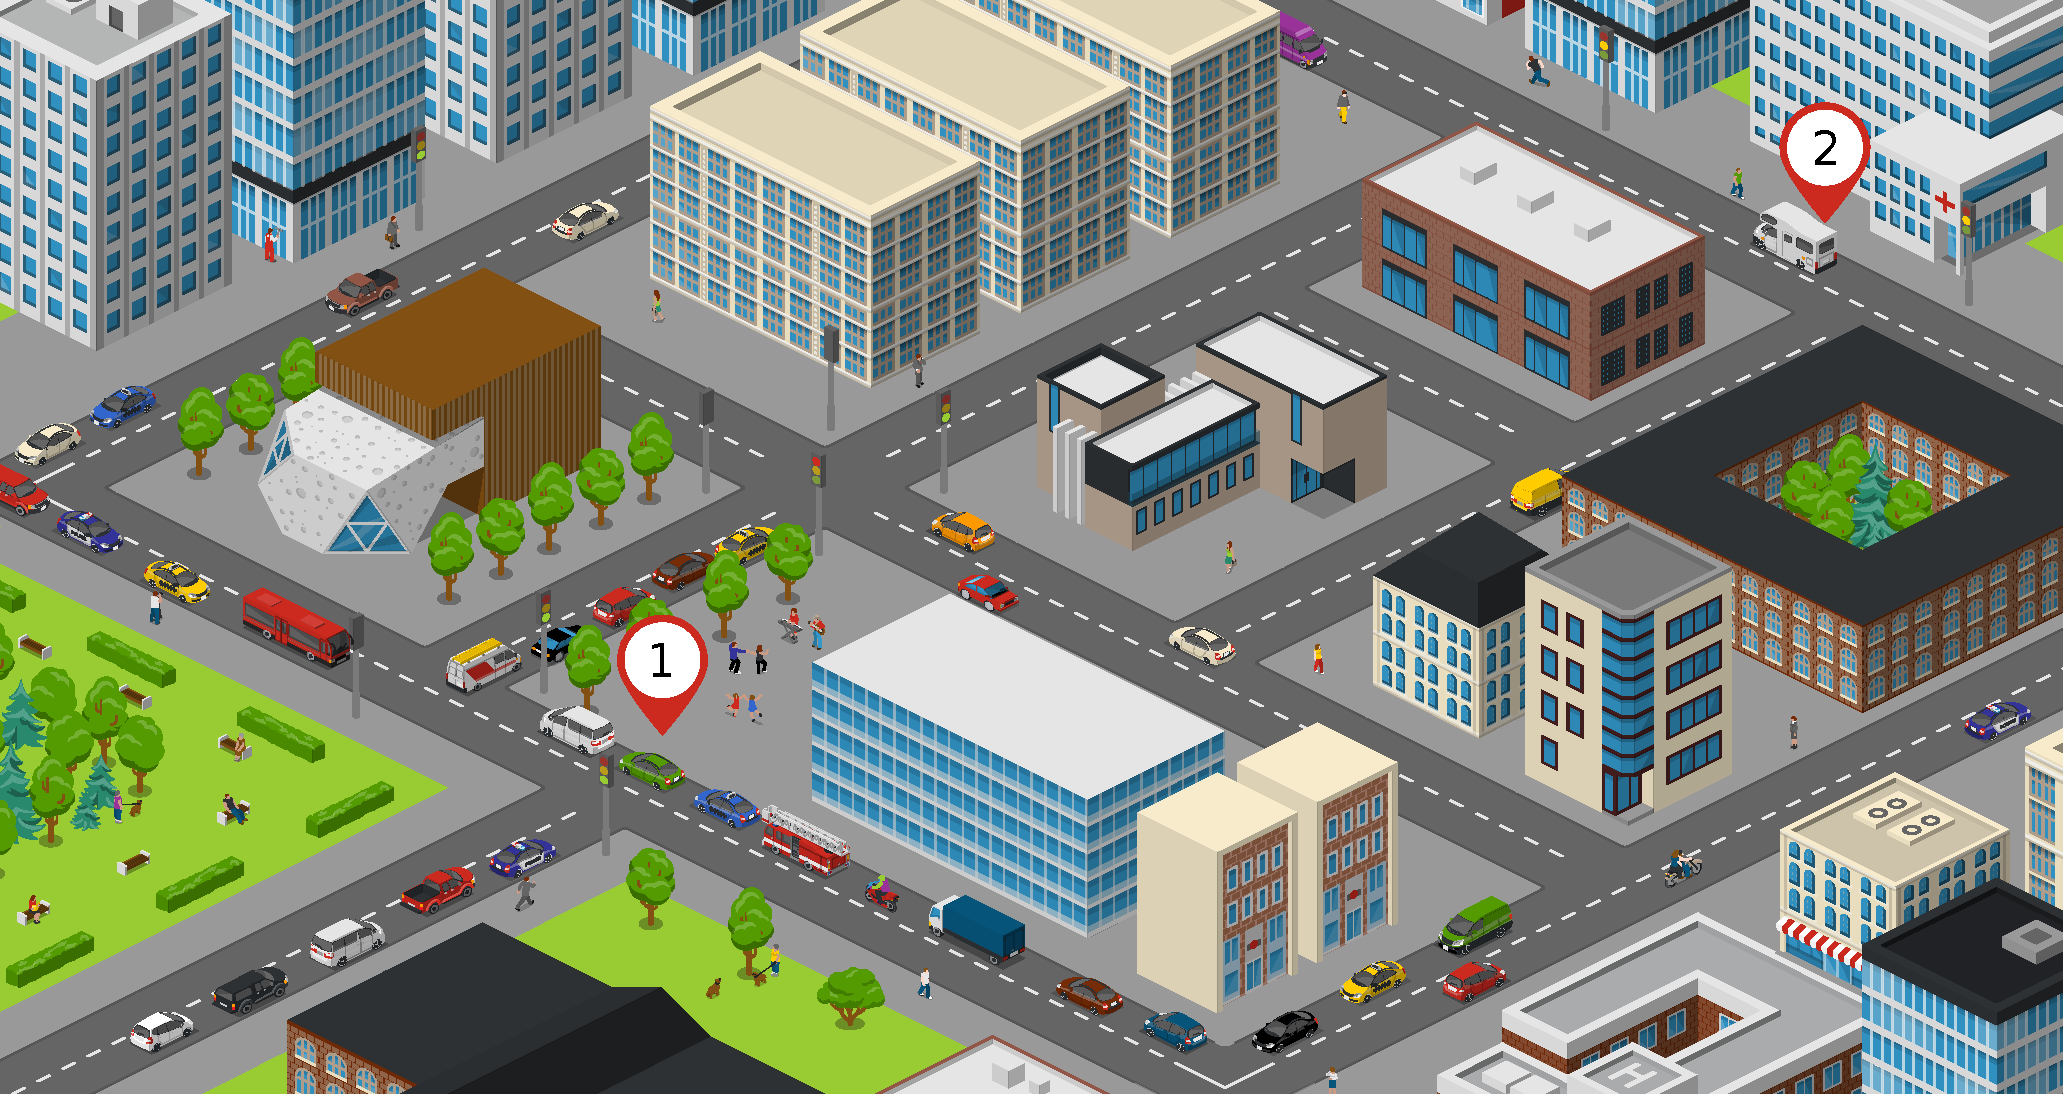
\includegraphics[width=1\textwidth]{parts/figuras/virtual-its-v2.pdf}
    \caption{1 represents a busy street with traffic lights and cameras, 2 is a less busy street that contains no road sensing infrastructure.}
    \label{fig:virtual_its_infrastructure}
\end{figure*}

Figure \ref{fig:virtual_its_infrastructure} shows an example of an application scenario. A busy street (1) contains several sensors on traffic lights, RSUs and other systems integrated to the road infrastructure. A less busy street can be observed in 2. On this street, it is possible to take advantage of the vehicles sensors to complement existing information that existing infrastructure sensors can't provide. Also, with shared data on the other roads, a driver or an autonomous vehicle can make smart detour decisions to avoid traffic jams.

With a data service that could provide real time data of only position and speed, ITS technology can offer, among other things: traffic monitoring and forecasting even in locations where there are no stationary traffic sensing units.

% ---
\section{Autonomous vehicles and sensors}\label{av-sensors}
% ---

According to the Society of Automotive Engineers (SAE International) J3016 standard, there are six levels of driving automation, from  “no automation” to “full automation” and they are summarized in table \ref{tab-levels}.

\begin{table}[htb]
\footnotesize
\begin{tabular}{|p{1.0cm}|p{3.0cm}|p{3.5cm}|p{3.3cm}|p{3.3cm}|}
   \hline
   \textbf{Level} & \textbf{Name}  & \textbf{Steering and Acceleration/Deceleration}  & \textbf{Monitoring of Environment}  & \textbf{Dynamic Driving Task} \\
    \hline
    0 & No Automation  & Human driver & Human driver  & Human driver \\
    \hline
    1 & Driver Assistance & Human driver and System & Human driver & human driver \\
    \hline
    2 & Partial Automation & System & Human driver & Human driver \\
    \hline
    3 & Conditional Automation & System & System & Human driver \\
    \hline
    4 & High Automation & System & System & System \\
    \hline
    5 & Full Automation & System & System & System \\
    \hline
\end{tabular}
\caption{J3016 levels of driving automation}
\label{tab-levels}
\end{table}

The more automated the system in table \ref{tab-levels}, the more reliant it becomes to sensor data. State-of-the-art AVs utilize a wide range of on-board sensors. High sensor redundancy is required for robustness and reliability in most of the vehicle tasks \cite{9046805}. Electric vehicles have and increasing number of sensors, as reference data points, the BYD Atto 3 has 5 cameras and the Tesla Model 3 has 9.

Sensor data provides critical information about the environment, the driving area, and potential obstacles in the vehicle path. The data collected by these sensors forms the basis for the autonomous vehicle's decision-making and control systems \cite{li2023learning}.

The different modalities of sensors address different aspects of environmental perception. For example, cameras are adept at sensing color without emitting signals for measurement, making them valuable for tasks such as traffic light detection. However, they are sensitive to changes in illumination and have limitations in obtaining depth information. 

Lidar and radar sensors, on the other hand, excel at measuring depth and distance to objects, providing critical 3D information that complements the data captured by cameras. Ultrasonic sensors, with their ability to detect obstacles and measure distance using sound waves, further enhance the sensor suite of autonomous vehicles.

% ---
\section{Simultaneous Localization and Mapping}
% ---

Simultaneous Localization and Mapping (SLAM) is a set of methods and algorithms that find vehicle location in a space reference frame while simultaneously mapping the given surrounding space \cite{Zheng2023}. This is critical to navigate and operate in unknown or dynamic environments, specially if existing maps or external localization systems are unavailable or connection is unstable.

SLAM combines sensor data, such as visual, inertial, and depth information. With this data it is possible to estimate the vehicle's pose and location and construct an updated map of the environment in real time. Using the self-generated map and continuous localization estimates, robotic systems can plan and execute trajectories, avoid obstacles, and interact with their environment in a robust and autonomous manner.

SLAM is critical for cooperative perception, as any shared perception message will contain location information of the vehicle and the perceived surrounding. If the vehicle location is imprecise, this will impact the localization of any detected objects.

Considering that Localization is the task to position the car relative to a reference frame in the environment, by having this shared reference frame, its possible to combine data from several different vehicles and apply that to a shared localization and mapping application.

%State of the art SLAM techniques can be categorized in several ways, one could categorize they by the used algorithms like Filter Based SLAM or Deep Learning Based SLAM.
When looking to State of the art SLAM techniques from the sensor point of view, they can be split in 3 types: visual SLAM, lidar SLAM, and multi-sensor SLAM. A recent SOTA comparison in \cite{garigipati2022} found that overall, Lidar-based methods generally outperformed visual SLAM in outdoor settings and with dynamic objects, benefiting from their broader field of view.

% ---
\section{Sensors}
% ---

The main types of sensor devices used for perception in the context of autonomous vehicles are described in the following subsections. 

% ---
\subsection{Radar}
% ---

Radar technology, short for Radio Detection and Ranging, is a detection system that uses radio waves to determine the range, angle, or velocity of objects. It was initially developed for military purposes prior to World War II. Radar systems can detect ships, missiles, vehicles, aircraft, and other objects by sending out pulses of high-frequency electromagnetic waves and observing the echoes that are returned. One of the advantages of this sensor is that velocity and position can be measured simultaneously based on the Doppler Effect.

In present days radar technology found a big number of applications, relevant examples for this work are: air traffic control, weather forecasting, traffic monitoring and autonomous vehicles. When used on autonomous vehicles, radar provides real-time data for obstacle detection, speed measurement, and collision avoidance. It can operate in various light conditions and can complement other sensors such as LiDAR and cameras to enhance vehicle perception systems.

Current standard frequency for Autonomous Vehicles by the European Telecommunications Standards Institute is between 77 and 81 GHz (ETSI TR 103 593 and \cite{ramasubramanian2018moving}). These frequencies are fast enough to provide the reaction time required by autonomous vehicles and are accurate up to a distance of 250 meters.

Notable radar limitations include susceptibility to jamming and electromagnetic interference, multiple Reflections and Clutter. Clutter refers to unwanted echoes or signals detected by radar systems from objects that are not the target of interest. These may include reflections from the ground, buildings, trees, and other static objects, as well as atmospheric phenomena such as rain and snow.

For comprehensive awareness, autonomous vehicles typically have six to ten radar sensors placed around them (with an exception in Tesla vehicles). In 2022, Waymo's self-driving taxi had six radar sensors, while Mercedes-Benz used eight radar sensors in their test vehicles.

% ---
\subsection{LiDAR}
% ---

LiDAR is an acronym for Light Detection and Ranging, it is a remote sensing method that uses light in the form of a pulsed laser to measure the distance between objects. The system determines the distance to an object by emitting light pulses and measuring the time it takes for the reflected pulses to return. 

This technology was initially developed in the 1960s, shortly after the invention of the laser. It was first used in military research (for satellite tracking) and meteorological tasks, like measuring clouds and pollution.

LiDAR has been applied across diverse fields over the years, besides autonomous vehicles, it has a big number of applications. Relevant recent usages are astronomy (Mars topology analysis and Navigation Doppler Lidar), Archaeology (Upano Valley sites) and Military.

The current state of technology employed in autonomous vehicles allows for a range of up to 400 meters. The sensor outputs the position and intensity of light reflected at a given point, allowing for the measurement of both distance and reflectance values. This information can be used to create a 3D point cloud of the vehicle's surroundings.

LiDAR is a significant component alongside cameras and radars and is favored for its precision in range measurement, which is crucial for detecting other vehicles, pedestrians, and various entities to ensure more safe traffic \cite{li2020lidar}.

In the literature, the biggest limitations of this kind of sensor are high costs, big volume of generated data management and bad performance with adverse surface types or under bad weather condition \cite{s23062972}.

% ---
\subsection{Cameras}
% ---

Digital camera technology is designed to capture optical images using photosensitive sensors to convert light into electronic signals that form digital images. Cameras operate by focusing light through a lens onto a sensor array that records the light intensity and color of the 3D space into a projected 2D image.

An image sensor array typically consists of a CCD (Charge-Coupled Device) or CMOS (Complementary Metal-Oxide-Semiconductor) image sensor. These two types of image sensors are widely used in camera technology. CCD sensors are preferred for applications where image clarity and detail are the priority, such as in astrophotography and high-end digital photography, due to their high-quality images and better light sensitivity.

On the other hand, CMOS sensors have a construction that enables independent reading of each pixel. This feature contributes to faster processing speeds and lower power consumption compared to CCDs. Therefore, CMOS sensors are particularly attractive for use in devices where battery life and rapid image capture are critical, such as mobile phones and some consumer-grade cameras.

The history of camera technology dates back to the early 1600s with the formal invention of the camera obscura (earlier experiments of the actual technology usage dates back to as far as 500 AD). Since then, significant progress has been made, particularly in digital imaging during the latter part of the 20th century. Initially used for artistic and documentary purposes, cameras quickly found applications in various fields, including science, security, entertainment, and more recently, in autonomous vehicle systems.

Compared to other sensors, cameras have very distinct features. They work for long and short range detection and have large field of vision and angular resolution. The cost can be high, in case advanced camera sensors with high resolution are being used, but can also be very low if simpler settings are used, especially when compared with LiDAR sensors.

Despite being critical components, cameras come with several limitations that can impact their performance and reliability, a few examples are: sensitivity to environmental conditions, like fog, heavy rain and night; limitations in perceiving depth; difficulties with direct sunlight and high lighting variations.

In autonomous vehicles, digital images provide visual information about the vehicle surroundings that other sensors cannot capture, like information from traffic lights or traffic signs. In recent years Tesla moved to a new program called Tesla Vision, in which it replaced radar and ultrasonic sensors by camera sensing, believing that the future in AV sensing is in image\footnote{https://www.tesla.com/support/transitioning-tesla-vision}.

As reference, we observe that new electric vehicles come equipped with an increasing number of cameras, the BYD Atto 3 has 5 cameras and the Tesla Model Y currently has 9\footnote{https://www.tesla.com/ownersmanual/modely/en\_us/GUID-682FF4A7-D083-4C95-925A-5EE3752F4865.html}.

% ---
\subsection{GNSS}
% ---

GNSS (Global Navigation Satellite System), commonly referred to as GPS (Global Positioning System), is a satellite-based navigation system that provides geolocation information to a receiver anywhere on the planet. GPS refers to the North American Global Positioning System, while GNSS refers to the International Multi-Constellation Satellite System. This means that it has access to other satellite systems, such as GLONASS, Baidu, Galileo, and others, in addition to GPS.

Initially developed by the United States Department of Defense in the 1970s, the technology was intended for military navigation. Since then, it has expanded vastly in its applications across various sectors.

The sensor system operates by using a network of satellites that transmit radio signals to receivers on the Earth's surface. These signals provide data on the satellites' location and the exact time the signals were transmitted. The GNSS receiver calculates its own position by measuring the time delay between receiving the signals from at least four satellites. This time delay helps determine the distance from each satellite. By determining the distance to multiple satellites, the receiver can triangulate its position in three dimensions.

Recent advancements have improved the accuracy of GNSS technology in civilian use to within a few meters. In autonomous vehicles, GNSS provides critical positioning data that supports other sensors, such as cameras and LiDAR, to create a comprehensive understanding of the vehicle's environment.

GNSS systems face challenges such as signal disruption or blockage in closed or dense environments, as well as vulnerability to signal interference and spoofing. While GNSS provides global coverage and has broad applications, these challenges can limit its reliability and performance in critical navigation and timing tasks.

% ---
\subsection{IMU}
% ---

Inertial Measurement Unit (IMU) sensing consists of a combinations of accelerometers, gyroscopes, and magnetometers that provide data used to track an object's acceleration, rotational motion, and orientation. IMU technology is currently used in a wide range of applications, including navigation systems, consumer electronics, robotics, and also in the field of autonomous vehicles. 

IMUs have an important role in autonomous vehicles by providing essential data for dead reckoning and improving the vehicle's ability to determine its position and orientation in situations where GNSS may be unreliable or unavailable, such as tunnels or urban canyons.

The sensor nature enables integration with other systems, such as GNSS, LiDAR, and radar, forming a comprehensive sensory network that significantly reduces the system's vulnerability to the failure of any single sensor.

However, this kind of sensor also have its limitations. Notable challenge are temperature sensitivity and drift errors in accelerometer and gyroscope readings, which can accumulate over time and lead to increasing inaccuracies if not regularly corrected or calibrated.

Not all autonomous vehicles use IMUs. For example, Waymo does not employ this sensor on their autonomous vehicles. Instead, they use a combination of LiDAR, radar, and cameras.

% ---
\section{Cooperative perception}\label{cooperative-perception}
% ---

In an abstract view, cooperative perception can be seen as the collaborative exchange and integration of data among system components to enhance their overall situational awareness beyond individual capabilities.

The concept has derived from research in vehicle-to-vehicle (V2V) and vehicle-to-infrastructure (V2I) communications. The shared perception approach allows robots and autonomous vehicles to collectively perceive and interpret environment data, significantly increasing the accuracy and reliability of the information derived when compared to isolated systems which rely solely on onboard sensors \cite{YU2022100023}.

Although cooperative perception technology has promising benefits, it also faces significant limitations. High bandwidth and latency requirements are necessary due to the real-time sharing of data among multiple entities. Furthermore, challenges such as data privacy, security, and integration of heterogeneous systems are ongoing fields of research. The effectiveness of the technology is limited in areas with poor network coverage or compromised network infrastructure due to its dependence on consistent connectivity.

The current SOTA methods in cooperative perception technology seek to address these limitations by optimizing data transmission mechanisms\cite{THANDAVARAYAN2023103655} and integrating machine learning algorithms to enhance data processing efficiency and accuracy \cite{xu2022v2xvit}.

Intelligent Transportation Systems (ITS) can integrate these advancements in cooperative perception technology to create more efficient, safer, and more responsive transportation networks. Through ITS, vehicles can communicate with each other and with traffic management systems, resulting in improved traffic flow, reduced congestion, and enhanced safety.

The use of cooperative perception in ITS is relevant because it enables a shared situational awareness. This awareness allows proactive traffic management and incident response strategies not only on the personal level for the vehicle but for the road infrastructure as a whole.

% ---
\section{Sensor fusion for ITS applications}\label{sensor-fusion-its}
% ---

In the same sense as cooperative perception, but at a lower level, sensor fusion is a method where data from various sources is combined to enhance individual measurements.

Current state of the art research on multi-sensor fusion systems for Autonomous Vehicles have a prevalence of three kinds of combinations in the literature: camera-LiDAR(CL), camera-radar(CR) and camera-LiDAR-radar(CLR).

Data fusion approaches can be categorized based on the abstraction level at which sensor data is integrated. According to \cite{s21062140}, when thinking about multi sensor data fusion, there are three primary data fusion classifications used in modern sensor systems: High-Level Fusion(HLF), Mid-Level Fusion(MLF), and Low-Level Fusion(LLF).

LLF is the most granular approach, also known as data level fusion, it consists of combining raw data from all sensors directly. This method is ideal for applications requiring high precision and extensive data detail, as it preserves all of the original sensor information. While it increases the potential accuracy and robustness of sensor interpretations, it also significantly increases the complexity of data processing and requires sophisticated calibration and alignment of sensors. It also generates a large volume of data that can be difficult to manage and process effectively.

MLF, also referred to as feature-level fusion, integrates data by extracting features from individual sensor data before combining them. This method balances between integrating raw data and processed results,  providing a moderate level of detail and processing complexity. It allows for better context retention than HLF by using raw data’s features rather than completely processed data. However, MLF requires large training sets for effective feature selection and can be challenging to calibrate accurately.

HLF works by first processing data from individual sensors, each of which independently performs detection or tracking algorithms. These results are then combined into a consolidated object definition. The main advantage of this approach is its simplicity, which requires less computation (since it is offloaded to the sensor systems) and less detailed understanding of the underlying sensor technologies. However, HLF can result in the loss of potentially valuable information, as only the processed results from each sensor are merged, discarding any raw data that may contain useful, subtle details.

The nature of sensor fusion presents complex challenges. With the large volume of data from diverse sensors, synchronization becomes imperative to ensure reasonable performance. Given that different sensors emit data at irregular intervals, they are subject to processing delays and transmission latency. If these factors are not properly addressed, they could result in miscommunication or error.

ITS represent a significant area where sensor fusion technology is extensively applied. Sensor fusion for ITS can combine multiple data sources like cameras, radars, and GNSS, to create a more comprehensive understanding of traffic scenarios.

A relevant example is in the context of ITS is Google Maps and Waze, which use data from a large number of users, along with input from mobile phone sensors (which are not necessarily the state of the art in sensing capabilities) and historical traffic data, to predict traffic levels and suggest optimal routes to users. These platforms are simple examples of ITS in action, where sensor fusion can facilitate real-time traffic monitoring and management.

% ---
\section{Simulation environment}\label{sim-env}
% ---


Considering the recent developments in autonomous vehicle technology, researchers need realistic simulations for training and evaluation of AI models and automotive operating systems. The security of V2X systems is also a growing concern, specially in the face of cyber attacks. For these reasons, simulation environments have and important role in analyzing the behavior of communication in V2X systems, and enabling research on topics such as jamming \cite{da2023radio} and spoofing \cite{mullertechnical}. 

Based on this premises, the CARLA simulator and Simu5G were selected for research experimentation. The CARLA simulator is used for physics and environment simulation and the Simu5G is used for network simulations. Both frameworks are open source and extensible, but none was designed with built-in features to integrate with one another. In this sense, a “simulation communication framework” was developed for this work.

Recent research \cite{cislaghi2023simulation} have successfully integrated CARLA and Simu5G by using Message Queues and a controller in each of the services. A similar approach was used and will be further explored in the chapters ahead.

\subsection{CARLA Simulator} \label{carla-sim}

The CARLA simulator, standing for Car Learning to Act \cite{MALIK2022742}, is a platform designed for autonomous driving research and development. It can create controlled and customizable environments for testing autonomous vehicle technologies. CARLA also supports a wide range of scenarios, including weather variations and different traffic conditions. Figure \ref{fig:carla_screenshot} shows an example of the rendered simulation.

\begin{figure*} [!ht]
    \centering
    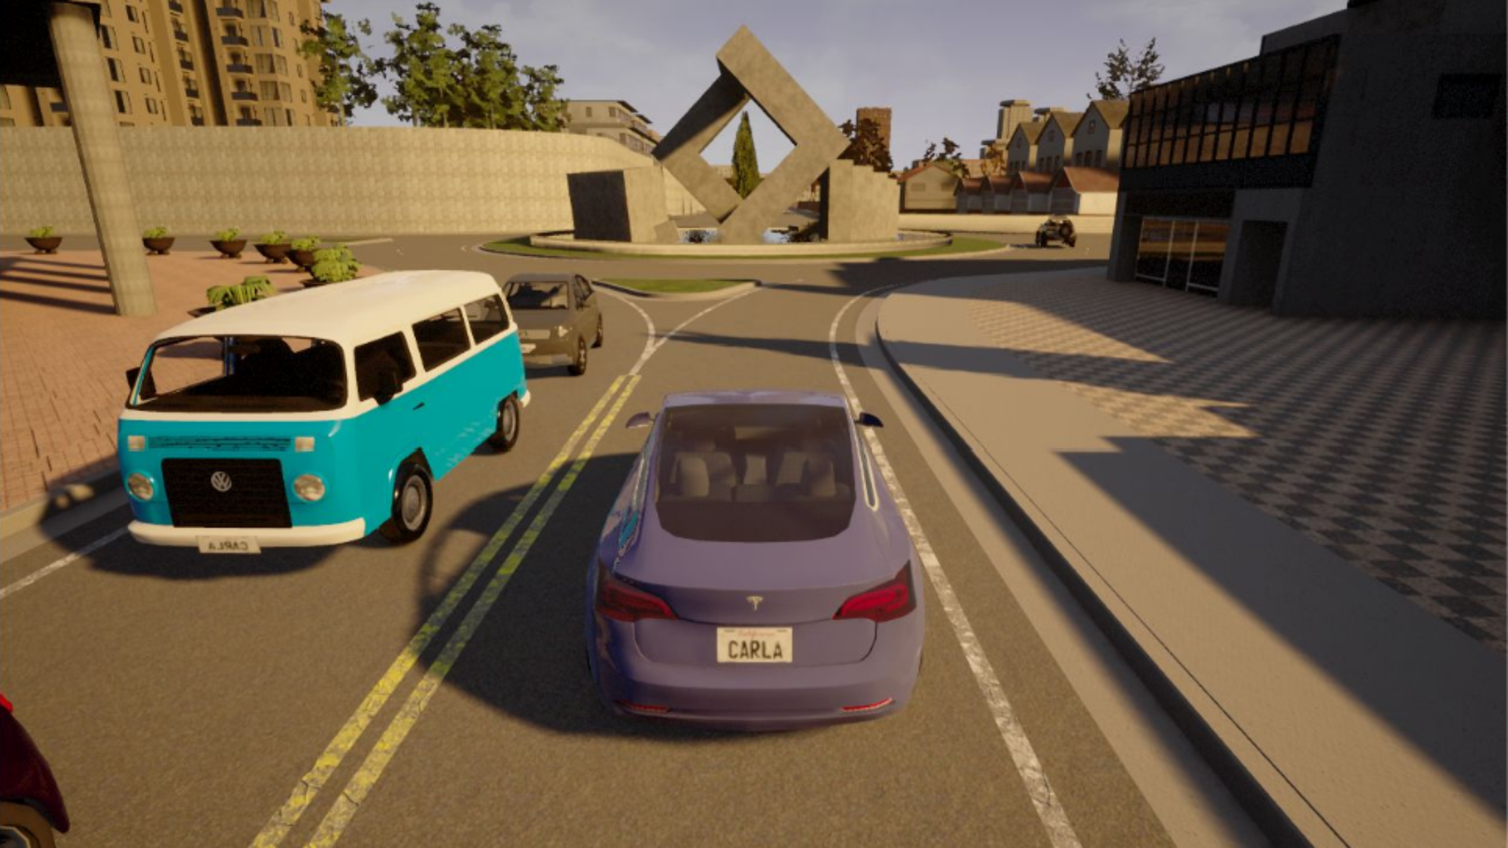
\includegraphics[width=0.80\textwidth]{parts/figuras/carla_screenshot.pdf}
    \caption{A screenshot of a simulation in CARLA. Carla is based on the Unreal Engine 4}
    \label{fig:carla_screenshot}
\end{figure*}

The core motivation for using CARLA is the requirement for risk-free, reproducible, and flexible testing platforms which traditional physical testing methods cannot provide. Its ability to integrate with major machine learning frameworks (as well as ROS robot operating system) and substantial community involvement\footnote{https://github.com/carla-simulator/carla} makes it a reasonable research tool.

\begin{figure*} [!ht]
    \centering
    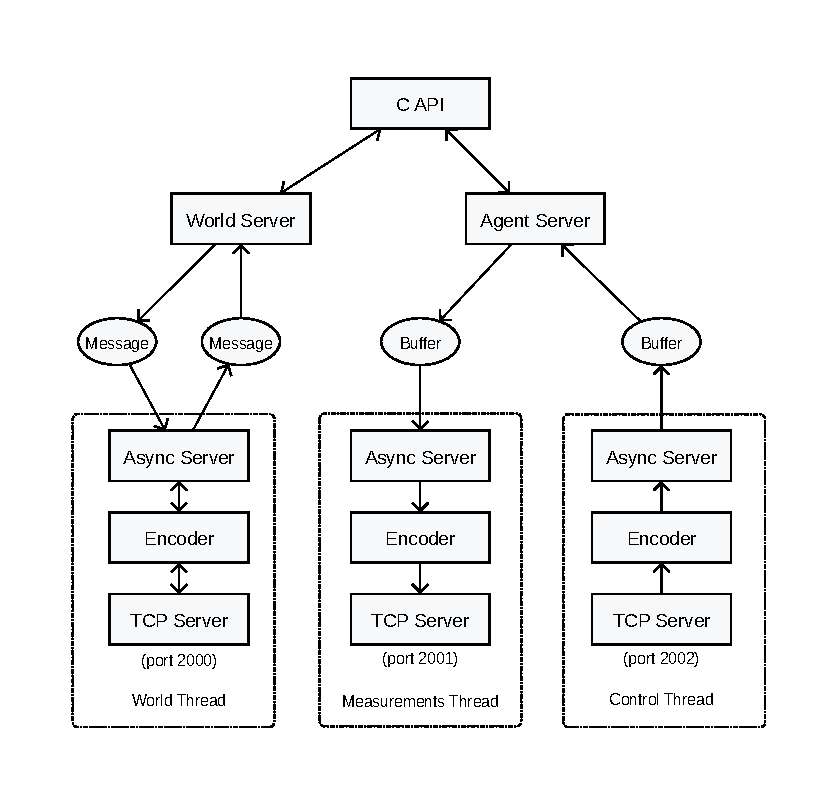
\includegraphics[width=0.70\textwidth]{parts/figuras/carla_architecture.pdf}
    \caption{CARLA architecture, from official documentation https://carla.readthedocs.io/en/stable/carla\_server .}
    \label{fig:carla_architecture}
\end{figure*}

Figure \ref{fig:carla_architecture} depicts the architecture of the CARLA simulator. It is primarily based on a server-client model, with the simulation running as the server and the external control managed by separate client instances. This server can be set up to accept multiple client connections, enabling collaborative testing environments.

The server can be accessed via TCP and has 3 interfaces, the world port, a control port, and the measurements port, each has a server behind which provide a different service.

The "World" server is responsible for controlling the overall simulation environment, while the Agent server has two threads: one dedicated to handling real-time metrics streaming(measurement port) and the other for interactive controls between clients and simulation(control port). This architecture ensures asynchronicity and control even with a considerable number of clients interacting with the server at the same time.

In CARLA, Actors are elements that perform actions within the simulations. These vary from vehicles to pedestrians, each created, managed, and removed through CARLA’s simulated world object, that is accessible within its client API. The essence of the actors lies in their detailed blueprints, which are templates defining attributes like vehicle color, lidar channels, or pedestrian speed. These blueprints are crucial for adding new actors to the simulation as they specify configuration preconditions and spawn behaviors for the Actors.

Finally, at the CARLA environment, sensors serve as the primary medium for data collection and environmental interaction for autonomous systems undergoing testing. A diverse array of sensors is supported, including standard cameras for RGB, depth, and semantic segmentation, GNSS, IMU Lidar and radar. As the sensors simulate real-world device functionality, they facilitate comprehensive testing in a controlled and realistic setting.

\subsection{OMNET++ and Simu5G}

OMNeT++ is an open-source simulation framework designed for network and distributed system simulations. It provides an infrastructure based on components that can be hierarchically nested, allowing researchers to construct the topology of their simulations in a dynamic manner.

The framework supports the implementation of both physical and application-layer network protocols through the use of various modeling techniques, including finite state machines and message passing for communication between components. It contains a graphical interface base on the Eclipse IDE \footnote{https://eclipseide.org/} that can assist in the design, execution, deployment, and analysis of simulation results. Figure \ref{fig:OMNET_IDE} shows an examples of a running experiment at the graphical interface. Network topology is presented at the center of the interface and the network profile is presented below. Network events are displayed sequentially and can be inspected for details.

\begin{figure*} [!ht]
    \centering
    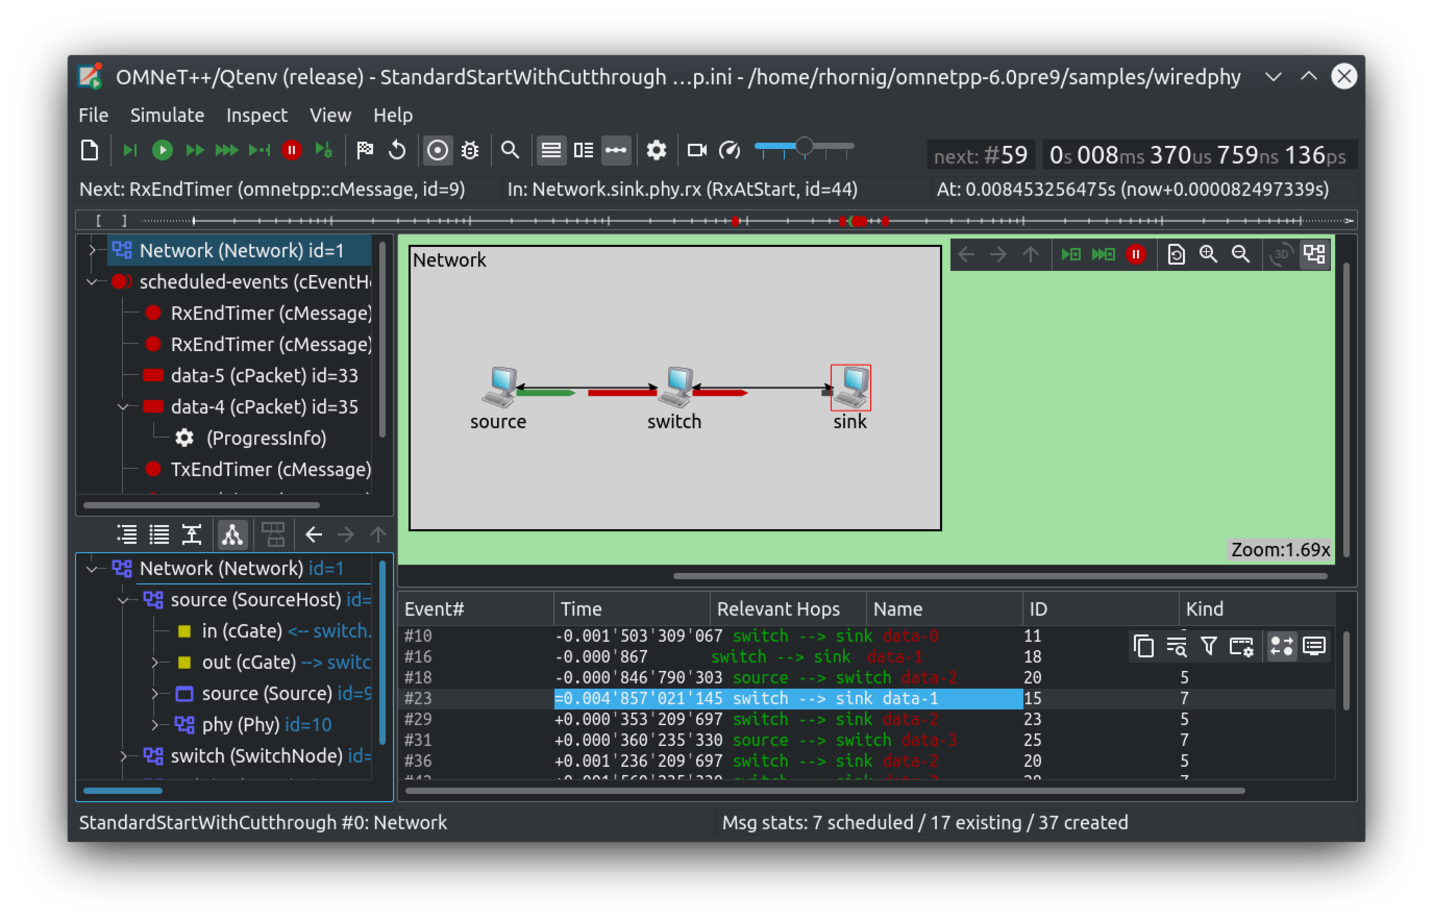
\includegraphics[width=0.75\textwidth]{parts/figuras/OMNET_IDE.pdf}
    \caption{A screenshot of the OMNET++ graphical interface from release 6. https://omnetpp.org/software/2020/11/03/omnet-6-pre9-released.html}
    \label{fig:OMNET_IDE}
\end{figure*}


Simu5G, on the other hand, is a library that extends the capabilities of the OMNeT++ simulator to model end-to-end behavior of 5G networks \cite{9211504}, including low latency, and high data rate communications. The library incorporates features such as dual connectivity, service-based architecture, and a wide variety of deployment scenarios from dense urban to rural settings, all within the scenario-based modeling provided by the OMNeT++ framework.

It specifically simulates the data plane of the 5G RAN (Release 16) and the core network. The library allows for simulation in both Frequency Division Duplexing (FDD) and Time Division Duplexing (TDD) modes across heterogeneous gNBs, ranging from macro to pico cell sizes, and it includes features such as handover support and inter-cell interference coordination via the X2 interface. 

Dual connectivity with LTE (eNB) and 5G NR (gNB) base stations is also supported, alongside 3GPP-compliant protocol layers. Realistic, customizable channel models are used for the physical layer, and the system supports resource scheduling in both uplink and downlink directions. Simu5G also supports numerous mobility models for user equipments, including those designed for vehicular mobility contexts.


% ---

% ---
% Capítulo com a proposta desenvolvida
% ---
% ----------------------------------------------------------
\chapter{Literature Review}
% ----------------------------------------------------------

This chapter presents a summary of current state of the art research and  works related to our proposed contributions with a focus on ITS and Cooperative Perception research.

\section{Intelligent Transportation Systems}

Within ITS applications, two big areas of research have have come to prominence. First, the current and future travel time prediction studies are helpful for route planning and traffic management. Second, there is a big number of studies on the construction of intelligent infrastructures, including smart cities, roadside devices, and IoT to improve communication performance and security. Other notable research is generally orthogonal to these two branches is also included to provide an overview of the field.

For travel forecasting \cite{chen2022constructing} and \cite{bhatia2022intelligent}, evaluate AI algorithms and mathematical progressions to predict travel times. \cite{haydari2020deep} reviews extensive literature on deep learning technologies for travel time prediction. For most of these works, real-time data is crucial for an accurate answer. In line with this, \cite{liu2018development} and \cite{wang2021trusted} propose models or approaches for data collection ranging from installing devices in vehicles to using mobile sources for data generation and training of AI algorithms.

An extensive review composed of 586 articles is done in \cite{kaffash2021big}. The article discusses big data algorithms and their applications in ITS, where the increasing amount of data requires advanced, data-driven approaches. The application of big data algorithms in ITS includes areas such as traffic flow prediction, travel time and route planning, and improving vehicle and road safety. Authors identify gaps in the field and show that the most used algorithms for ITS are based on deep learning methods.

In contrast to the described above, the second research branch proposes architectures for developing an intelligent infrastructure. The research's primary focus is installing embedded devices on the roads. In \cite{zhu2018big}, a cheap embedded device to popularize ITS applications is proposed. Other works, such as \cite{wang2021trusted} and \cite{guillen2021intelligent, garg2018deep, liang2019deep}, propose using data from existing sources, such as the use of IoT systems, images from security cameras, and others.

To further explore what can be achieved by a combination of modern technologies to improve ITS, \cite{dai2019artificial} investigates the applications of AI, edge computing, and caching technologies to improve the efficiency of ITS systems. RSUs are used to offload the computing closer to the network edge. The AI decision-making process provides a more efficient resource allocation and optimizes the network routing plan. With the inclusion of edge offloading and caching, latency and communication time are drastically reduced.

In \cite{tanwar2019tactile} authors experiment with a non-orthogonal Multiple Access network to meet current industry and standards and government regulation. Authors model the end-to-end latency under the designed architecture and analyze the reliability concerning the interruption probability of the network. Statistical analysis is used to model different latency components including transmission, processing, and propagation latency. Results show that its possible, with a combination of wifi and 5g, to keep latency under 5ms.

A survey on the latest advancements in Blockchain for IoV is done in \cite{Mollah_2021}. Authors evaluate the integration of of these technologies to address ITS communication challenges. The potential benefits of this combination are enhanced data security, increased reliability, and system transparency. While recognizing the promise of the convergence of blockchain and IoV in enriching the intelligence and security of transportation systems, it also highlights the existence of several practical adoption challenges that need to be overcome. These include issues related to scalability, energy consumption, privacy concerns, and lack of regulation.

In \cite{bao2021review} authors define digital twin in transportation and its possible applications. Similarities and differences between traffic simulation and digital twin are discussed. The article explores modeling vehicle driving behavior and environment simulation with the Digital twin. A three layers architecture is proposed, including data access layer, calculation and simulation layer, management and application layer.

Looking at the new 5G communication standard, \cite{gohar2021role} discusses the role it has in enhancing smart city functions, with a particular focus on ITS. It explains how 5G technologies are critical to realizing the concept of smart cities by providing high-speed connectivity, low latency, and the ability to handle a large number of connections. Particularly for ITS, the article discusses how 5G will enhance the interconnectivity of different transportation modes, improve traffic management, and increase overall transportation efficiency. 

To further improve AV and ITS capabilities, \cite{elghazaly2023high} explores the use of High Definition maps. A review of the state of the art of HD maps uses in the various functions of autonomous driving systems is presented. Authors discuss the AV components relying on Map Data, like SLAM, scene understanding, motion prediction and planning modules and how HD maps can greatly improve AV capabilities. Furthermore, HD maps and GNSS data can be fused, offering robust and precise localization services to AVs.

Considering the above articles, an important highlight is that at this moment there is no research on building virtual infrastructures that feed ITS and traffic management systems with AV data in real-time.

\section{Cooperative Perception}


In \cite{s22155535} the authors summarize multi-sensor fusion methods, communication technology, and shared perception strategies. The impact of communication cost and robustness of vehicle positioning errors is analyzed. The authors argue that to achieve autonomy levels above 3, it is necessary to leverage advanced sensing technology, edge computing, communication, and other technologies to build a cooperative perception system. This work also reinforces the idea that the future lies in V2X applications, supported by 5G communication technology.

Another recent review took place in \cite{10208208}, the work summarizes the applications of multi-sensor fusion classification strategies in cooperative perception. It proposes a multi-sensor fusion taxonomy for autonomous driving perception and classifies fusion strategies into symmetric and asymmetric fusion with seven subcategories.

\cite{xu2022v2xvit} examines the potential of V2X communication to enhance the perception performance of autonomous vehicles. The authors propose a novel vision Transformer architecture, called V2X-ViT, which combines data from multiple vehicles' Lidar sensors and achieves state-of-the-art performance results compared to similar techniques that employ intermediate fusion. The article considers both an ideal communication channel and a noisy setting, where pose error and time delay are both considered. No network-specific experiments were developed.

In their work, the authors of \cite{Li_2023} address the issue of intermediate fusion in order to account for the possibility of Lossy Communication channels on V2V communications. The LC proposal is designed to accommodate real-world scenarios in which there are Doppler shifts introduced by fast-moving vehicles, interference generated by other communication networks, and dynamic topologies caused by routing failures as well as various weather conditions. 

An additional work that attempts to address lossy communication scenarios is presented in \cite{ren2024interruptionaware}. Instead of implementing intermediate fusion, the authors develop a prediction model to extract multi-scale spatial-temporal features based on V2X communication conditions, thereby capturing the most significant information for the prediction of the missing information.

In \cite{THANDAVARAYAN2023103655}, authors propose baseline mobility-based generation rules for cooperative perception messages with mechanisms to control the redundancy of the information and reduce channel overhead. The proposed techniques improve perception, reduce channel load, and enhance scalability for all cooperative perception communications.

To Address offline datasets for AI model training, \cite{xu2023v2v4real} creates a dataset specifically for V2V cooperative perception research. Three cooperative perception tasks are introduced with benchmarks for model evaluation. According to the authors, biggest challenges in cooperative detection include GPS error, asynchronicity, and bandwidth limitation.

In \cite{v2vformer} a multimodal transformer model is introduced for cooperative perception. This new model employs lidar and camera fusion from different vehicles to achieve SOTA cooperative perception performance. The transformer integrates point-based and voxel-based features into a single 3D representation.

To address the some inherent challenges in cooperative perception such as the loss of semantic information, perception errors, \cite{song2024spatial} proposes improving vehicle pose calibration. An object association approach named context-based matching is used, which calibrates multi agents pose to improve shared perception precision. Object association precision is achieved with decimeter-level relative pose calibration accuracy.

To further facilitate the development of research in the field, \cite{carletti2024ms} presents a new co simulation tool that allows physical and network simulations (integrates CARLA, OpenCDA, and ns-3). The framework facilitates analysis of  vehicular networks under various V2X technologies and enables evaluation of AIML-enabled autonomous driving applications leveraging realistic sensor data.

In the topic of safety \cite{safety} proposes a method for expanding the field of view for autonomous vehicles by using edge infrastructure sensors (e.g. RSU systems). The "Infrastructure cooperative autonomous driving" system demonstrated an improvement in safety speed of 17\% and a reduction in collisions in simulated scenarios.

Considering the large volume of sensor data generated recently by both autonomous vehicles and edge devices, \cite{10470399} proposes the use of a Spatial and Temporal Clustering algorithm which not only reduces the communication payload between vehicles by clustering perceived objects across AVs but also optimizes the use of communication resources. The work presents significant enhancement in the efficiency of vehicle-to-vehicle communication networks, increasing information reception by 10\% and reducing communication payload by approximately 41\% compared to previous ETSI standards.

in \cite{cislaghi2023simulation}, authors have successfully integrated CARLA and Simu5G to simulate vehicle teleoperation. Vehicle sensor data was sent to a remote controller that would transmit steering and acceleration commands to the vehicle.

Based on the above literature review, evidence suggests that ITS and Cooperative perception areas share a significant number of articles with parallel applications. For instance, in both fields there are articles that investigate the usage of algorithms and optimization of the communication channel for scalability purposes.


% ---

% ---
% Capítulo de resultados
% ---
% ----------------------------------------------------------
\chapter{Methodology }
% ----------------------------------------------------------

% [FROM INTRODUCTION:] Given this scenario, the following research questions will be evaluated: Is it possible to collect the Connected Vehicles data with minimal impact on the vehicle's embedded system? What is the feasibility to emulate a generic "plug and play" module that would work in any vehicle of this type? At scale, is it possible to use this data for improving vehicle sensing capabilities and traffic monitoring ?

In order to answer the research questions presented in the introduction, two sequential works are presented in this chapter. Firstly, the feasibility and impact of additional data collection from Autonomous vehicles is evaluated in a simulated environment. After the first experiments facilitate data collection, a traffic monitoring solution is experimented with.

After the the data collection experimentation, a research framework is developed based on related works to experiment with shared perception in V2V and V2X scenarios.


\section{AV data collection}

In this section we evaluate the impacts of a data acquisition model on AV concerning local processing, memory and storage.

The experiment was built on top of the CARLA simulator. CARLA contains a client-server architecture where the server runs the simulation computation and rendering. The client is responsible for information collection and interaction in the simulation world through "Actors", as previously presented in subsection \ref{carla-sim}. In this setup, two computers were used, one for the simulation server and one for the client.

To establish mechanisms for persistent and pervasive data collection for the presented environment, two scenarios were considered: (i) collect data from sensor actors, which are managed by the simulation server, and offer callback utility functions directly to the CARLA client, and (ii) collect data directly from CARLA’s underlying data layer, using application performance management (APM) tools.

Both computers shared the same local network. Communication between client and server was established through CARLA's Client library, leveraging its TCP socket setup across default ports: 2000, 2001, and 2002. This setup enables asynchronous encoding of messages using Protocol Buffers (Protobuf), to enhance efficiency in data transmission and networking operations. 

The source code is available on GitHub\footnote[7]{https://github.com/av-data-research-group/carla-data-collection}. The Carla Client operates on a personal laptop with the following specifications: Ubuntu 22.04 Operational System, 6.5.0-26-generic kernel, Intel i7-13650HX with 14 cores and 2.6 GHz base frequency, 32Gb RAM DDR4, 1 TB M2 SSD storage. The vehicle agents used in the simulation are available at the CARLA challenge\footnote[8]{https://leaderboard.carla.org/leaderboard/} and also possess github repositories.

In \cite{etsi2019intelligent}, 3GPP published a standard for a cooperative perception Service (CPS) and cooperative perception Message (CPM), the CPM describes all kinds of sensor data and confidence levels to be shared between vehicles.  Message size will scale up with the amount of sensors data attached and fusion or processing level of the present data.
 
To simplify the collection process and measurements in the present experiments, saved data only includes sensor output. CPM standard data format is not used as added metadata would not present a big influence in data volume. CPM will be considered for future work exploring communication experiments.

The document also cites a Frequency and Content Management entity, which determines the optimal CPM generation period and number of perceived objects and regions to be included in the CPM. That has an important impact in respect to the channel usage. Since in this stage of experimentation we are using raw sensor data and no perceived objects, we arbitrarily defined a period of 3 seconds of frequency for sensor data collection.

In order to precisely monitor Memory and CPU consumption, the python client process was monitored by its current PID. At the tests done with the APM server software, its process was also monitored and memory and CPU usage were summed. The Ubuntu System Monitor and a combination of the following shell commands were used: \mintinline{shell}{top -p PID}, \mintinline{shell}{cat /proc/PID/statm}, \mintinline{shell}{ps faux | grep PID}, \mintinline{shell}{pmap -x PID} and \mintinline{shell}{docker stats}. CPU usage will be expressed in percentage relative to the system CPU.

\begin{figure*} [!ht]
    \centering
    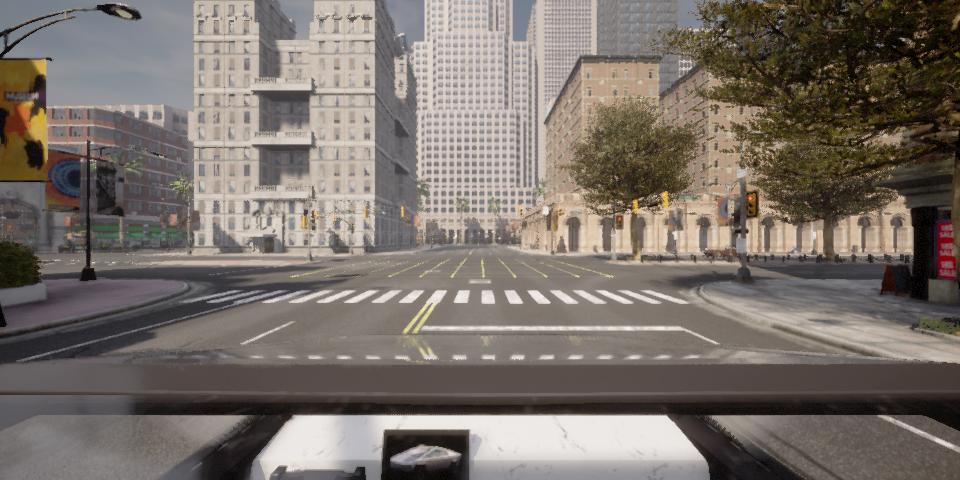
\includegraphics[width=0.8\textwidth]{parts/figuras/simulation-capture.png}
    \caption{A camera capture of the simulation. This camera was attached to the top of the car, and placed facing "front" relative to it.}
    \label{fig:simulation-screenshot}
\end{figure*}

Figure \ref{fig:simulation-screenshot} shows an example of a collected image from a vehicle camera in the simulation. Camera pose didn't reproduce its positioning in autonomous vehicles in the real world, as that is not relevant for measuring the system impact. An arbitrary positioning was used to help simulation monitoring, for example, to check if the vehicle was working as expected, didn't collide, among other problems that could happen during the experiment.

Table \ref{tab:my-table_1} presents memory and CPU consumption data for a single vehicle with 3 sensors that was created and integrated into the existing traffic manager of the simulation environment. In this simulated environment, the Elastic APM python agent creates several objects for monitoring and introspection, the memory spent is more than double the memory collected directly from the sensors.

\begin{table}[!htb]
\centering
\scalebox{0.83}{
\begin{tabular}{|l|l|l|l|}
\hline
    Usage                                       & Memory       & CPU  & Memory difference \\ \hline
without any data collection  & 29.0 MB & 0.44\% & - \\ \hline
with client data collection   & 38.9 MB & 0.55\% & 9.9 MB  \\ \hline
% 54.3 + 50.9 client + apm server memory values
% 0.57 + 0.1 client + apm server cpu values
with profiling data collection & 105.2 MB & 0.67\% & 76.2 MB  \\ \hline
\end{tabular}
}
\caption{Total memory and CPU comparison between collection methods. The simulation server is not accounted for.}
\label{tab:my-table_1}
\end{table}

Increase in CPU usage for the profiling solution was smaller than anticipated, our main hypothesis for this is that we are only monitoring a small number of objects (3 sensors) and the load is more memory and I/O based (for logging reasons). Total storage used after 1 hour of navigation was 441 MB, accounting for the images of the 2 cameras and 1 Lidar sensor.

New electric vehicles come equipped with an increasing number of cameras, the BYD Atto 3 has 5 cameras and the Tesla Model 3 currently has 9. To further evaluate the system load in respect to these kind of sensors only, we evaluated CPU and RAM usage against an increasing number of cameras. The cameras used a default setup of 960x480 resolution and 120 degrees field of view. Results are presented in Table \ref{tab:my-table_3}.

\begin{table}[!ht]
\centering
\scalebox{0.83}{
\begin{tabular}{|l|l|l|l|}
\hline
\# of cameras      & Memory       & CPU  \\ \hline
1  & 34.1 MB & 0.57\%  \\ \hline
2  & 38.4 MB & 0.82\%   \\ \hline
3  & 41.5 MB & 1.04\%  \\ \hline
4  & 44.3 MB & 1.19\%   \\ \hline
5  & 46.4 MB & 1.42\%  \\ \hline
6  & 48.0 MB & 1.58\%   \\ \hline
7  & 49.4 MB & 1.76\%  \\ \hline
8  & 51.2 MB & 1.95\%  \\ \hline
9  & 52.7 MB & 2.13\%  \\ \hline
\end{tabular}
}
\caption{Total memory and CPU usage for an increasing number of cameras, both increase linearly with the number of cameras.}
\label{tab:my-table_3}
\end{table}

To experiment with SOTA self driving models, Table \ref{tab:table2} presents impact on memory and CPU from collecting data for a Transfuser \cite{chitta2022transfuser} agent, the winner of one of the CARLA Challenges event. Sensor setup was reproduced from the authors github repository\footnote[9]{https://github.com/autonomousvision/transfuser/} containing 3 cameras (with higher resolution than previous baseline experiment), one lidar sensor, an IMU, a GNSS and a speedometer. A total of 7 sensors. As reference, for the Transfuser model training, each camera has, in addition to RGB, depth maps and semantic segmentation data.

\begin{table}[!ht]
\centering
\scalebox{0.83}{
\begin{tabular}{|l|l|l|l|}
\hline
    Usage                                       & Memory       & CPU  & Memory difference \\ \hline
without extra collection  & 29.4 MB & 0.4\% & -  \\ \hline
with sensor data collection   & 45.8 MB & 0.91\% & 16.4 MB  \\ \hline
% 58.8 + 50.4 (client + apm server memory values)
% 1.07 + 0.2 (client + apm server cpu values)
with profiling data collection & 109.2 MB & 1.09\% & 79.8 MB   \\ \hline
\end{tabular}
}
\caption{Total memory and CPU comparison between data collection methods for the Transfuser agent. Total sensor count in the CARLA simulator: 7. Simulation server is not accounted for in used memory.}
\label{tab:table2}
\end{table}

The same baseline model was used for navigation (not the Transfuser model), so the usage without the data collection in practice is the same. We can observe that the memory spent in the sensor data collection method increased around 20\%, this can be attributed to the growth of sensors on the vehicle. On the other hand, the memory from the APM data collection tools kept being much more significant, even though it didn't scale with the number of sensors like it did in the first experiment. For this experiment, the total storage used after 1 hour of data collection was 3.1 GB, This big increase in used memory is attributed to the increase in amount of sensors, number of cameras and camera resolution. Lidar setup didn't change between experiments.

To better understand the impact this system would have on a vehicle in the real world, we considered the Delphi Audi zFAS, which is a central driver assistance controller released in 2018, for Audi's A8 model. The controller owns a 4 GB SDRAM, DDR3L-1866, so with the transfuser setup (7 sensors) that translates to 1.1\% of total memory usage with the direct sensor collection, and 2.6\% with the APM data collection, a neglectable impact on a 6 year old controller. Additionally, the camera test still shows a feasible expenditure with 9 cameras: 52.7MB or 1.32\% of the total controller memory.

Autonomous vehicles have security and decision modules that need to access data with minimum latency. For this reason, CPU and memory assets must be rationalized as much as possible, the presented sensor data collection mechanism is able to meet that necessity.

In a nutshell, the costlier performance of the APM solution was expected due to the software evaluation infrastructure built around it. In physical vehicles, on the other hand, the extra load will be less than that presented in this work, considering that instead of a python profiler, a profiler is used at the vehicle operational system level.

The increase in amount of storage needed for the extra module is relevant as we show that for the transfuser model, this would be around 3GB for 1 hour. Camera and lidar data are raw and represent the biggest part of this volume, with 2.8GB dedicated to the 960x480 resolution images from the 3 cameras.

\section{A traffic monitoring experiment}

Considering that starting code is available for data collection, an additional data collection experiment was designed to take advantage of it.

In order to evaluate a simple traffic monitoring application, three "monitor vehicles" were placed in the simulation. For each vehicle, GNSS and speedometer sensor data was collected in the same way it was done in the previous experiment.

At the CARLA simulation, a map called Town10HD\_Opt was selected\footnote{https://carla.readthedocs.io/en/latest/map\_town10/}. This map's road network consists of a grid layout, including numerous different junctions and traffic lights.

A light and a heavy traffic scenario were considered, one with only the three vehicles in the simulation, allowing for top speed in the selected map, and one with the monitor vehicles and another 100 cars, to examine the heavy traffic scenario.

\begin{figure*} [!ht]
    \centering
    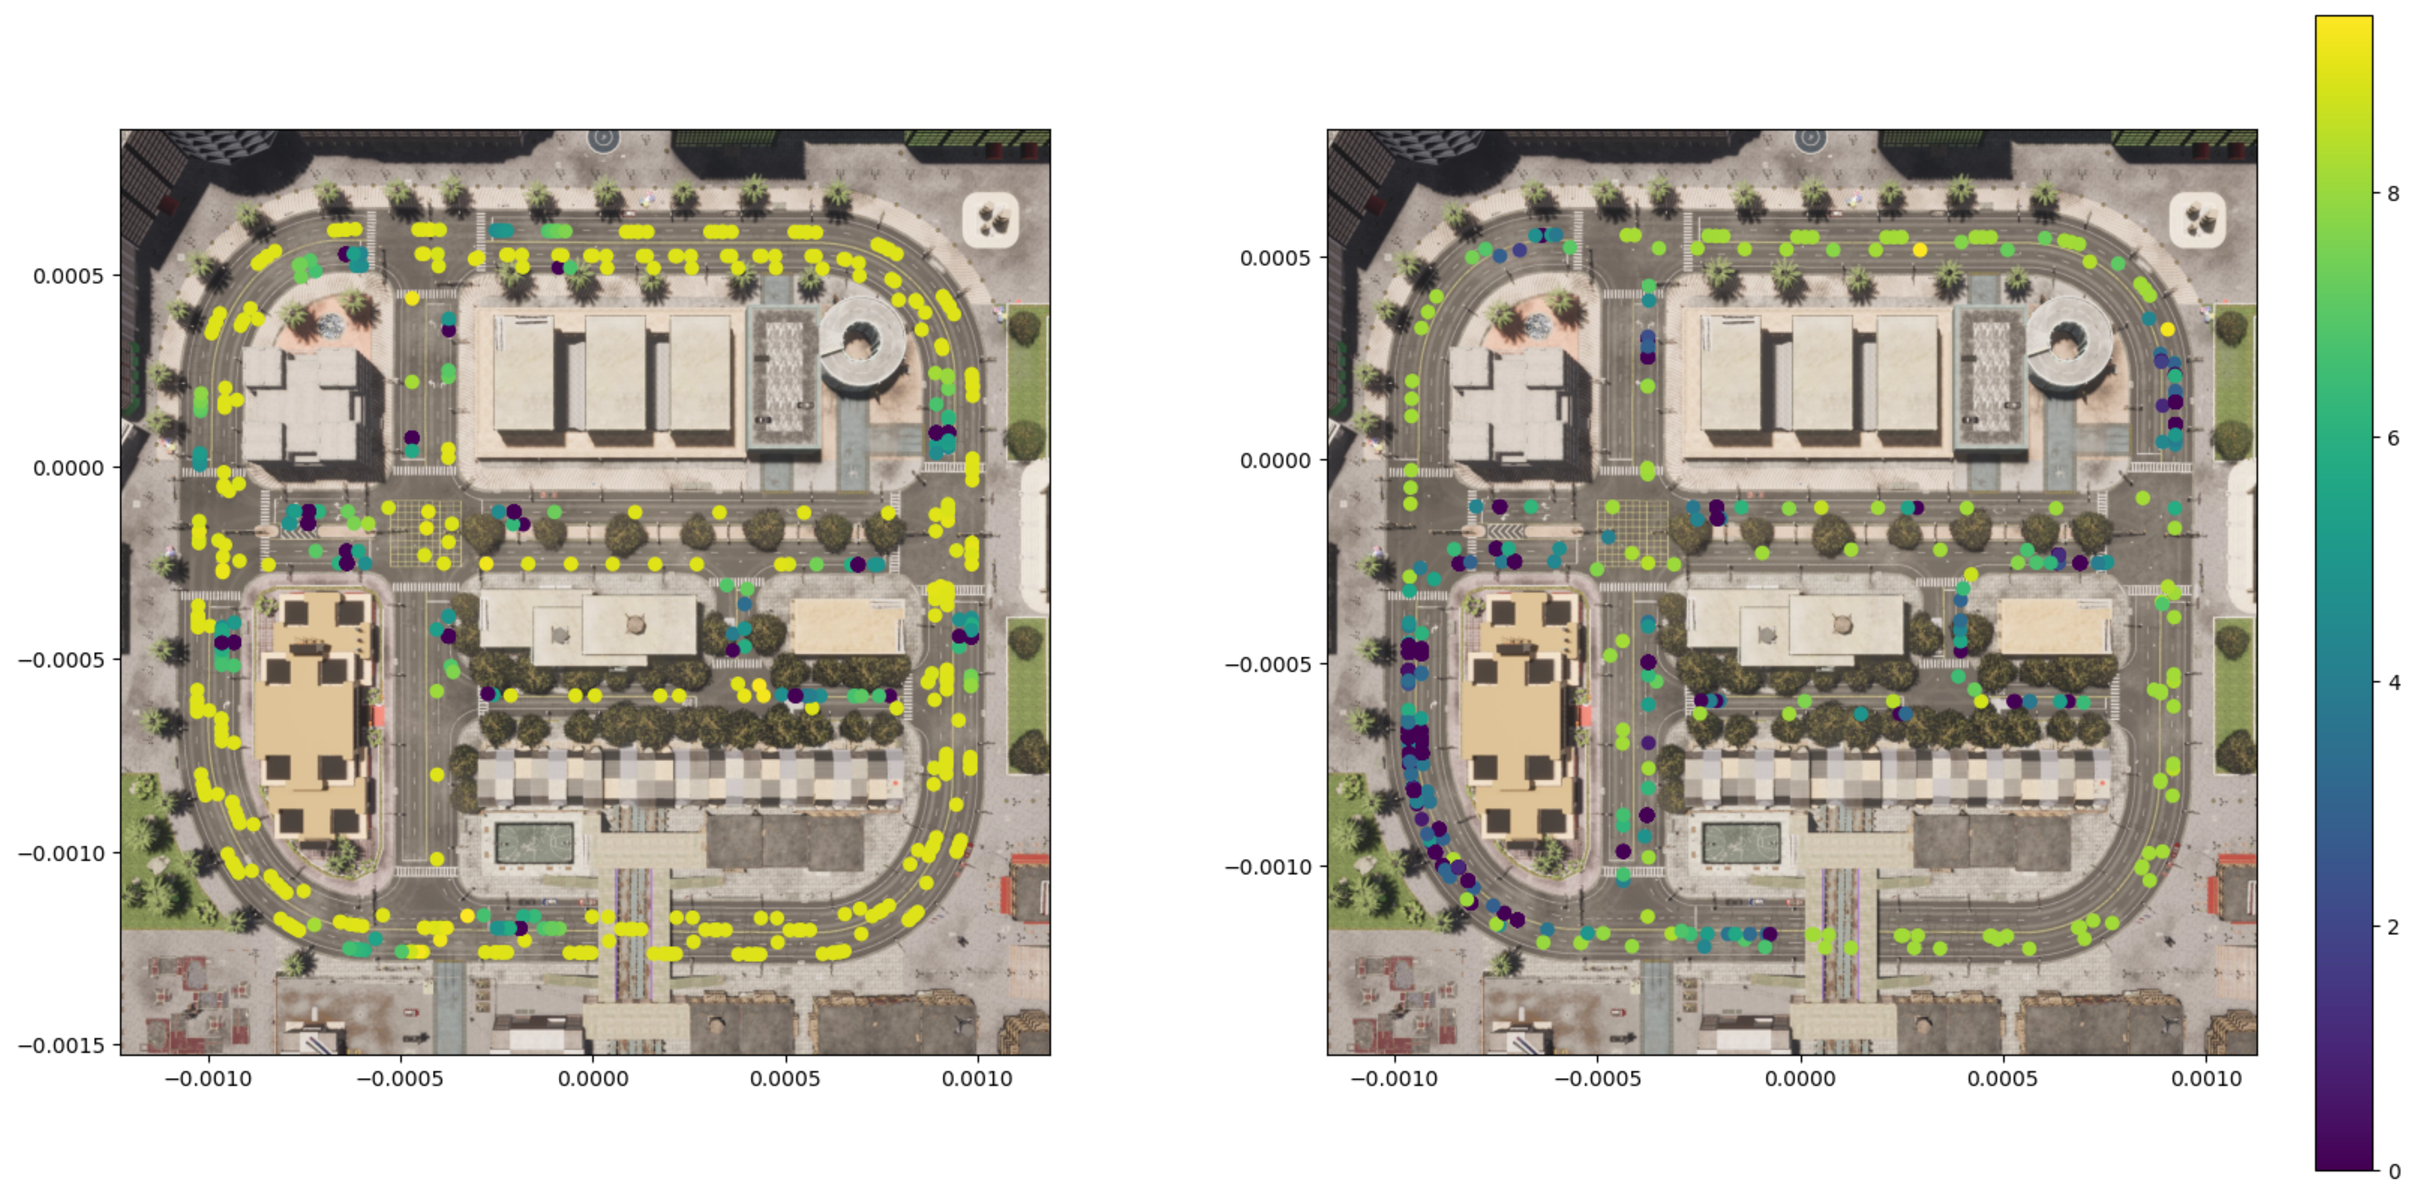
\includegraphics[width=0.9\textwidth]{parts/figuras/traffic-comparison.pdf}
    \caption{Traffic comparison, on the left the light traffic simulation, and on the right the heavy one. Points represent the vehicle location and the speed during collection step. Right color map is represented in meters per second.}
    \label{fig:traffic-monitoring}
\end{figure*}

Each vehicle built a log of the collected data, the log was monitored in real time and data was collected for 20 minutes. At the end of the simulation, map data was fused with the GNSS and speed data from the vehicles to generate the proposed traffic monitor.

Figure \ref{fig:traffic-monitoring} depicts the experiment end result. Its possible to observe that even in the light traffic scenarios, some points of the road have a lower mean speed. This points are present in junctions or traffic lights.

Another thing that was expected was the low average speed even for the light traffic scenario (~8.5 m/s or 30.6 km/h). This happened because the selected map represent a "downtown" location, consisting of several junctions and traffic lights, that would naturally lower the speed of passing vehicles.

As expected, in the heavy scenario situation, traffic light and junctions are the places with the biggest impact, its possible to observe a large traffic jam on the lower left corner of the map. Considering the simplicity of the generated code, it can be reused to evaluate light and heavy in all other CARLA maps.

If a minimal number of vehicles share this kind of data with a single, centralized server, its possible to have real time speed data with a reasonable error. The error rate increases with the decreasing of number of vehicles, as data gets "old" until another vehicle passes by the location to metrify speed again.

\section{Data transmission simulation}

In order to create the network experiments part of the cooperative perception simulation, we built a new application for communication simulation on top of previous experiments code. These new experiments do not use APM methods for data collection, and rely solely on CARLA`s sensor data implementation.

The new addition takes advantage of the Carlanet project \cite{cislaghi2023simulation}, in which Omnet and CARLA communication is implemented as a message queue with ZeroMQ.

\begin{figure*} [!ht]
    \centering
    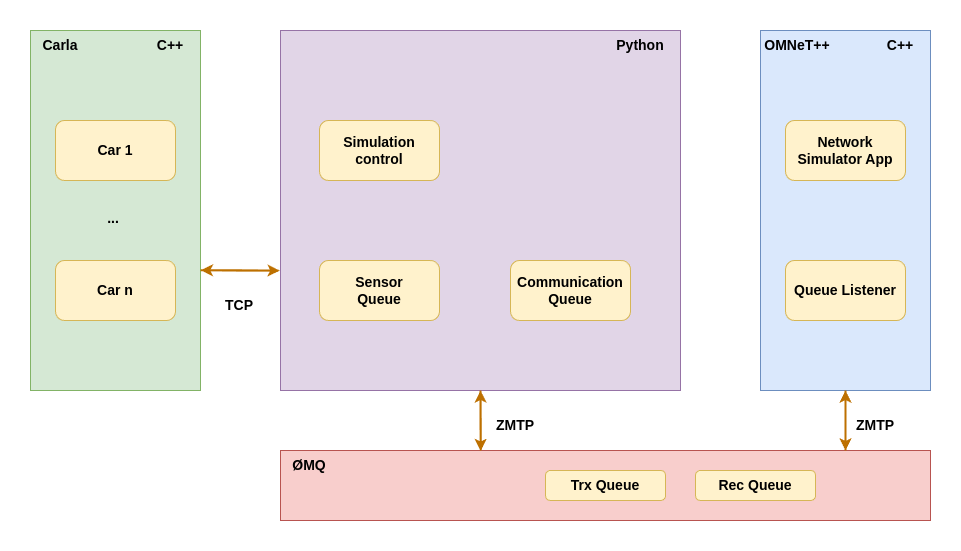
\includegraphics[width=0.9\textwidth]{parts/figuras/implementation-dissertacao.drawio.png}
    \caption{Block diagram containing the simulation framework components. Carla and experiment communicate via TCP and Omnet++ communication happens through ZeroMQ.}
    \label{fig:block-diagram}
\end{figure*}

As a significant amount of stack has been added to the experiment code, Figure \ref{fig:block-diagram} portraits the new overall setup. Communication with CARLA maintains the TCP standard with ports 2000, 2001 and 2002. When sensor data is available for transmission, or when the vehicle controller is asked for, sensor data is sent to OMNET++ through a transmission queue for network simulation. 

Default format for data transmission in the Carlanet setup is json messages, so when camera image data is transmitted, it has to be base64 encoded and then decoded as utf-8 to text, as bytes are not serializable in json format. An example of the json message is presented below in "Code" \ref{json:example}.

\begin{lstlisting}[caption={json message example},label={json:example}]
{
   "message_type":"GENERIC_RESPONSE",
   "simulation_status":0,
   "user_defined":{
      "msg_type":"VEHICLE_DATA",
      "camera_data":"gHx8/4F9ff+BfX3/gX19/.../gX19/",
      "actor_positions":[
          {
             "actor_id":"carlaNodeCar_1",
             "position":[
                325.1853942871094,
                1.9907456636428833,
                0.0019066429231315851
             ],
             "rotation":[
                -0.010655094869434834,
                0.06594514101743698,
                -0.00012207029067212716
             ],
             "velocity":[
                6.835569858551025,
                0.008157790638506413,
                8.010864007701457e-07
             ],
             "is_net_active":true
          }
      ]
   }
}
\end{lstlisting}

To keep both simulations synchronized, a "Simulation step" message is also exchanged between the simulations. At every simulation step, vehicle location and speed are sent to Omnet++. This is needed to correctly execute the 5G network simulations.

With the initial communication setup done, we reproduce the traffic monitoring experiment with location and speed data being transmitted from the vehicles to a 5G antenna placed in the center of CARLA`s TOWN01, the smallest map available.

The antenna is connected to a Remote Service Agent that sits in the python part of the code. When a new data message arrives, it performs network simulation (from car to antenna) at Omnet++ and forwards it to the experiment Receiving Queue for the Remote Agent to process. Once in the Receiving Queue, the remote service 
saves it to the local file system for processing by reusing code from the traffic monitoring experiment.

The following Sequence Diagram in Figure \ref{fig:sequence-diagram} represents how the experiments were performed. An initial configuration phase is done where all the simulators are started and configured. Omnet++ contains the trigger to start the entire experiment, after started, it triggers the experiment configuration both in itself and in carla, where the configured Actors are placed and vehicle control is configured.

\begin{figure*} [h!]
    \centering
    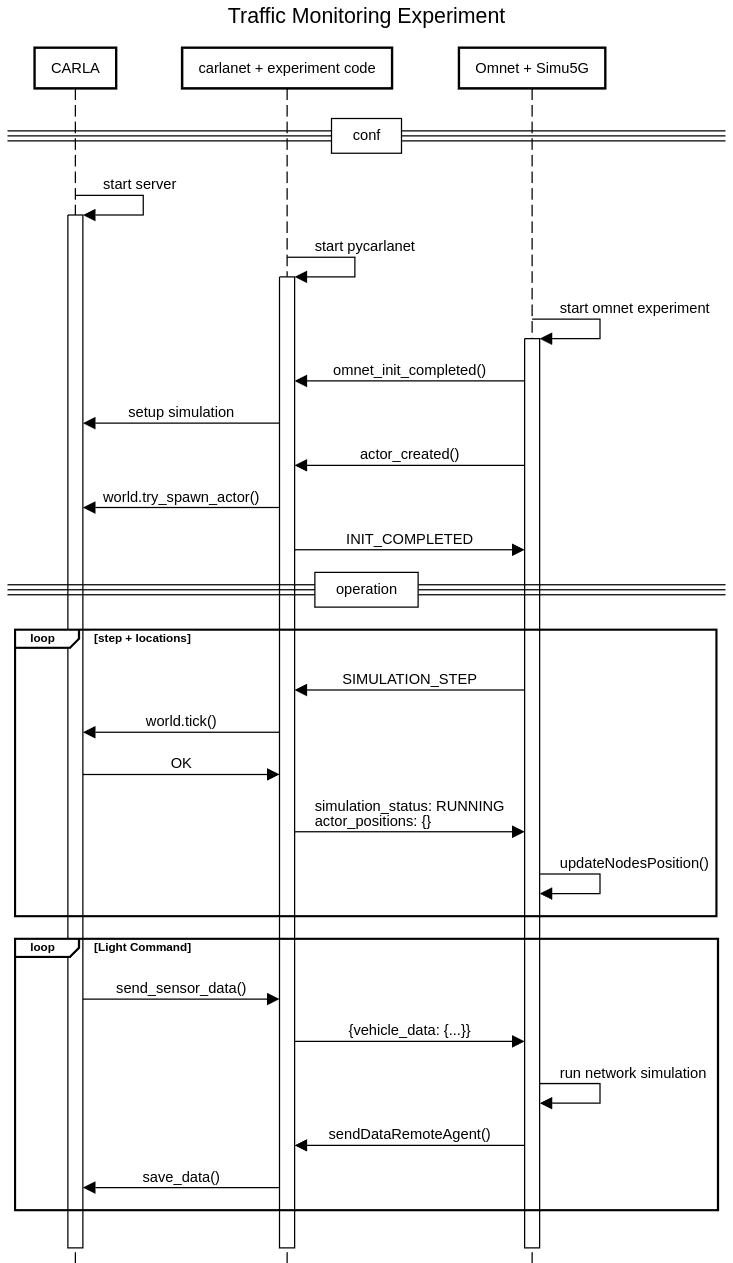
\includegraphics[width=0.5\textwidth]{parts/figuras/traffic monitoring sequence diagram.png}
    \caption{Sequence diagram representing the data flow in the experiment application. After an initial configuration stage, 2 communication loops are executed: One for simulation synchronization and other for data sharing.}
    \label{fig:sequence-diagram}
\end{figure*}

Two communication loops are then initiated, the "Simulation step" and the "Vehicle data" messages start being exchanged by using the ZeroMQ Service.

Traffic monitoring experiment is run for TOWN01, with a remote data service to represent an ITS traffic management system, again with 0 and 100 cars.

Results show the same standard as previous traffic monitoring experiment: average speed around traffic lights drop significantly when the map is full of cars. 

Results can be seen at Figure \ref{fig:traffic-monitoring-network}. datapoints are sparser even though the same number of monitor cars were used, that is due to the fact that the collection average time for each location and speed was increased from 3 to 9 seconds, in adaptations from the initial code to the Carlanet standard.

\begin{figure*} [!ht]
    \centering
    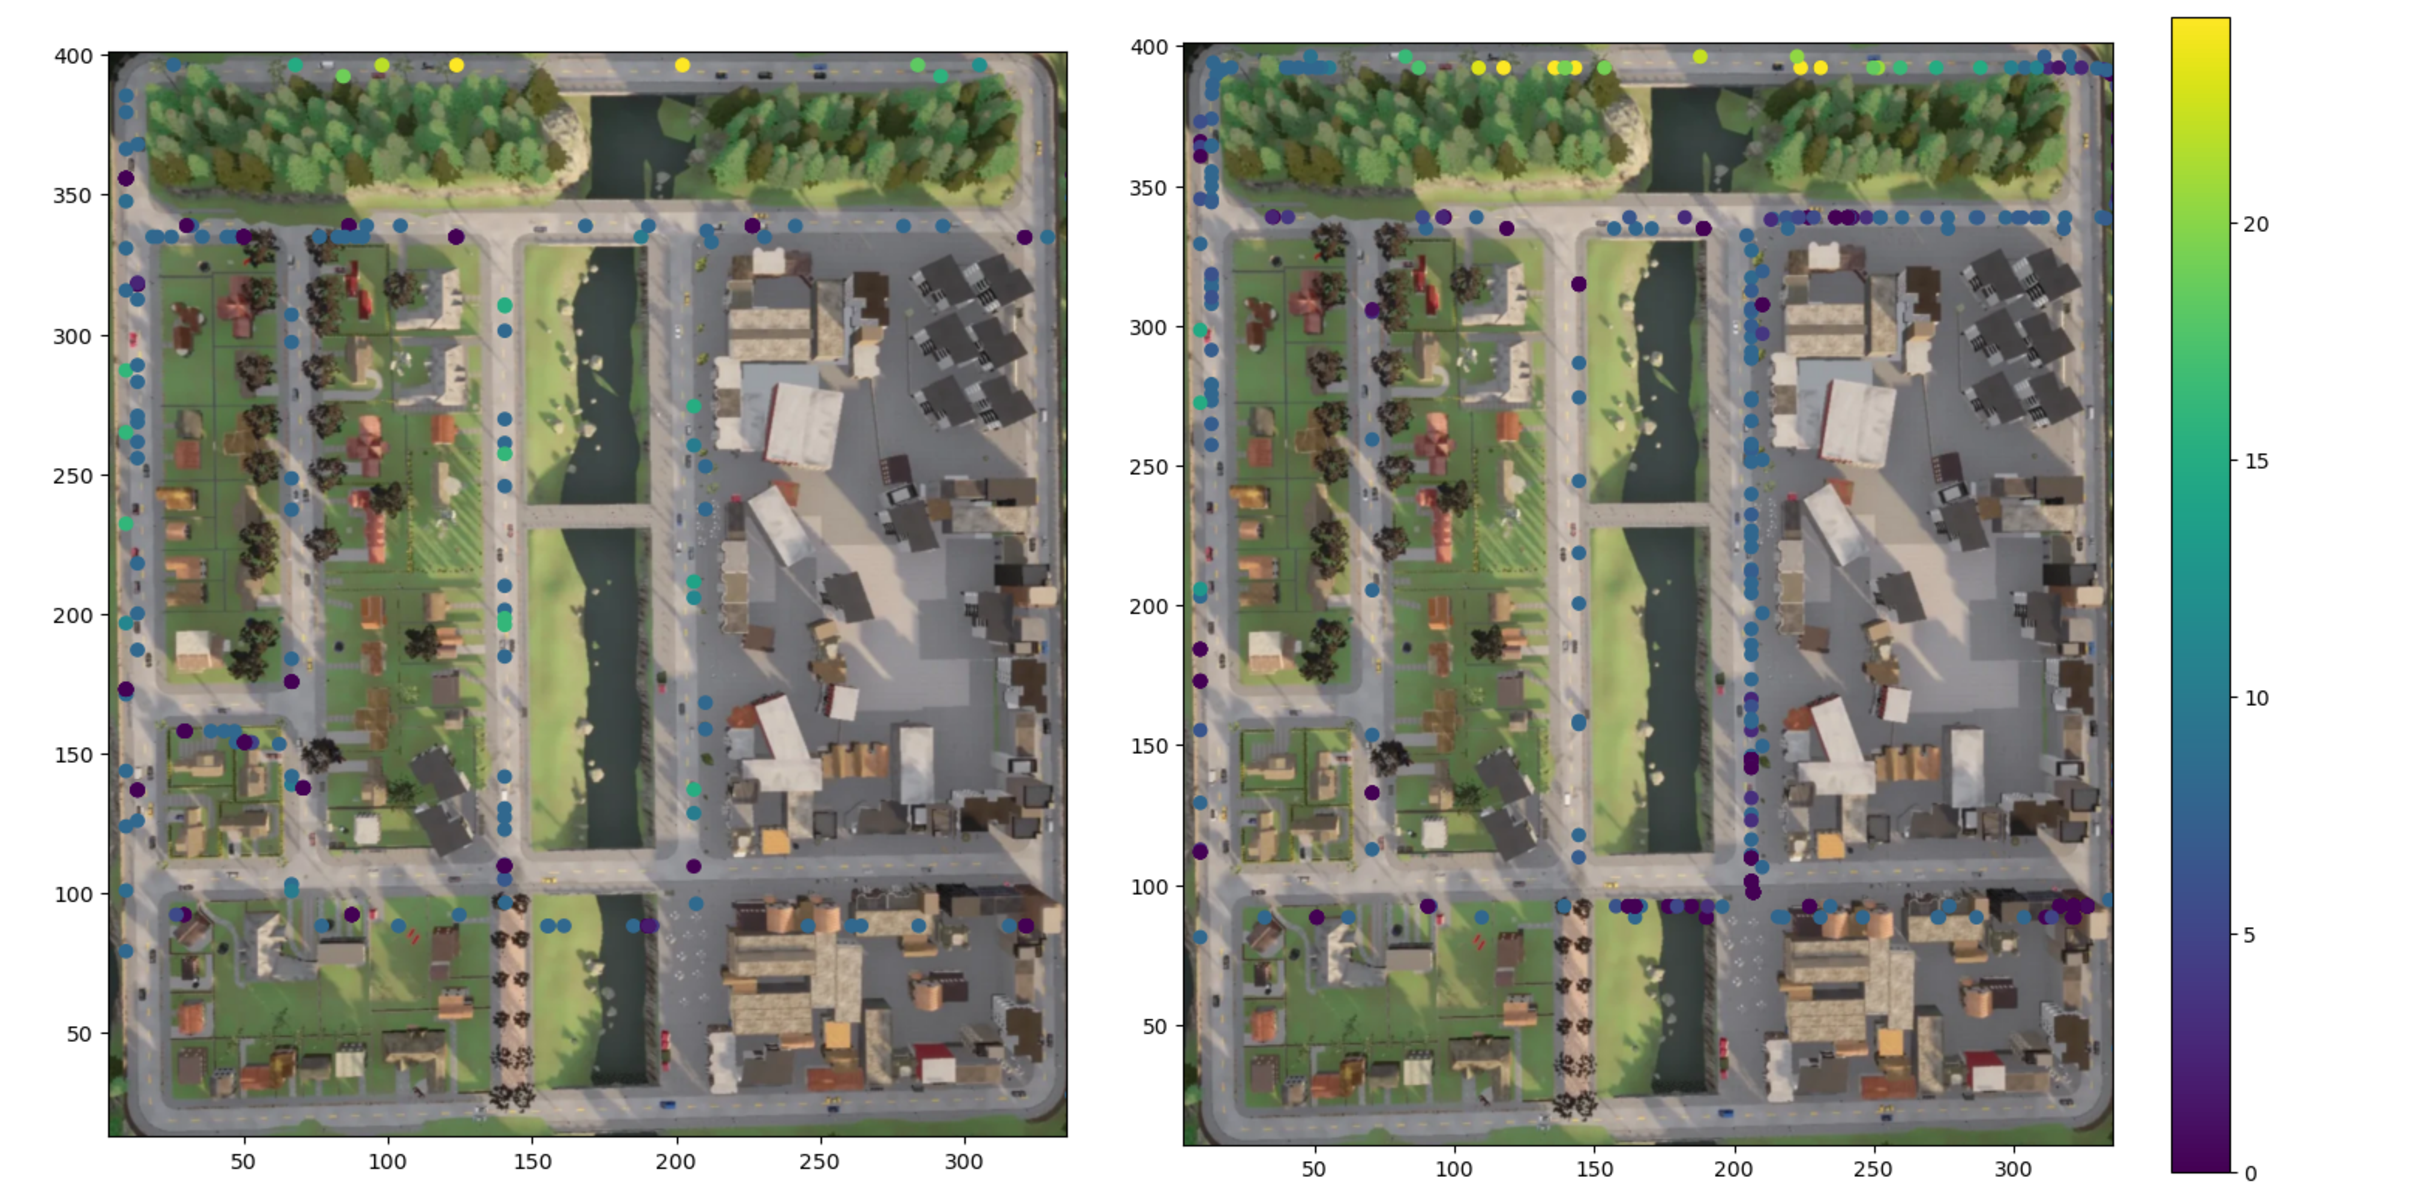
\includegraphics[width=0.9\textwidth]{parts/figuras/traffic-comparison-network.pdf}
    \caption{Traffic comparison, on the left the light traffic simulation, and on the right the heavy one. Points represent the vehicle location and the speed during collection step. Right color map is represented in meters per second.}
    \label{fig:traffic-monitoring-network}
\end{figure*}

Average speed was 18 km/h at the "No traffic" simulation and 10.8 km/h at the "High traffic" one. A thing to note is that Town01 is actually bigger than Town10, so an addition of 100 cars didn't have the same impact as it had in the previous traffic monitoring simulation.

\begin{figure*} [h!]
    \centering
    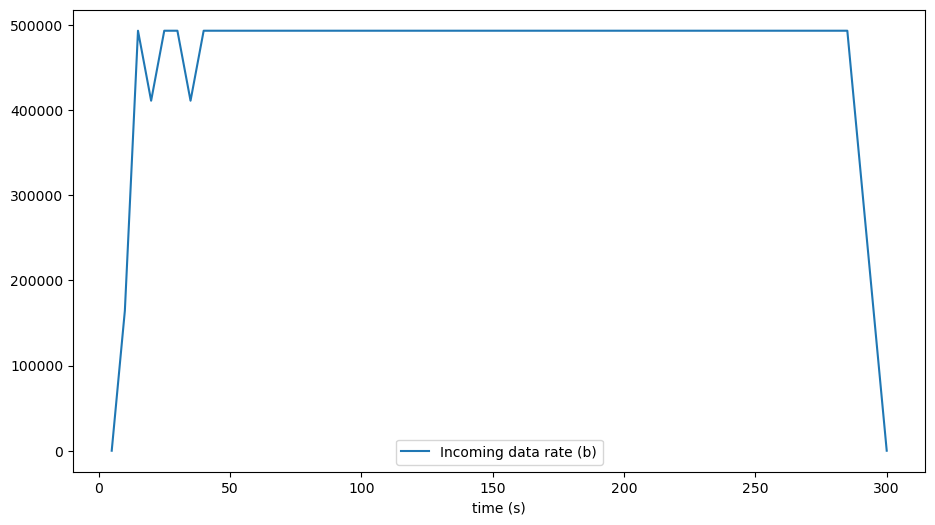
\includegraphics[width=0.7\textwidth]{parts/figuras/bitrate-1-car.png}
    \caption{Bit rate of a single vehicle during simulation time. Two messages are exchanged, Simulation step and traffic monitoring.}
    \label{fig:bitrate-1-vehicle}
\end{figure*}

In an additional experiment made to measure channel usage, figure \ref{fig:bitrate-1-vehicle} shows the Bit rate of the data transmissions from a single car for around 6 minutes of simulation: A total of 61,68 KB/s considering both Simulation step and traffic monitoring messages.

Our hypothesis for the first fall in the Bit rate after an established connection is occlusion or some sort of signal interference that was not purposely added to the simulation.

Considering that a 5G antenna capacity is 10 Gbps, both messages account for 0.049\% the maximum channel usage. If a dedicated antenna is considered, a single one is capable of receiving messages from 2040 vehicles at the same time.

Current B5G/6G research estimate big improvements with bitrates getting up to 100 Gbps, further increasing the feasibility of a virtual data infrastructure for traffic monitoring purposes.

\section{Cooperative Perception simulation framework for V2X Security experiments}

Building upon our previous data collection and transmission experiments, we developed a integration framework between CARLA and Simu5G simulators to enable cooperative perception testing focused on V2X cybersecurity. This integration addresses the critical need for realistic simulation environments that can model both complex traffic scenarios and 5G network communications simultaneously, particularly when evaluating security aspects like jamming and spoofing attacks.

The integration architecture, called B5GCyberTestV2X\_CARLANet, is the central connection point between CARLA and Simu5G. This framework enables vehicles within the CARLA environment to share sensor data through simulated 5G connections, creating a bootstrapped environment for cooperative perception algorithms under various security threat scenarios.

Within B5GCyberTestV2X\_CARLANet, several key submodules work together to facilitate the operation and programming of use case scenarios. Figure \ref{fig:B5GCyberTestV2X} shows the system architecture. The "Data" submodule collects information from sensors incorporated into the CARLA simulator, sending this information simultaneously to the TX submodule and the "Fusion" submodule. Meanwhile, the "Control" submodule manages vehicle actuators within the CARLA environment, ensuring precise control over vehicle behavior based on cooperative perception inputs. Any algorithm can be used with the control submodule, including CARLA's auto pilot feature. This setup creates a closed feedback loop where vehicles can share sensor data, process information from other vehicles, and adjust their behaviors accordingly.

\begin{figure*} [!ht]
    \centering
    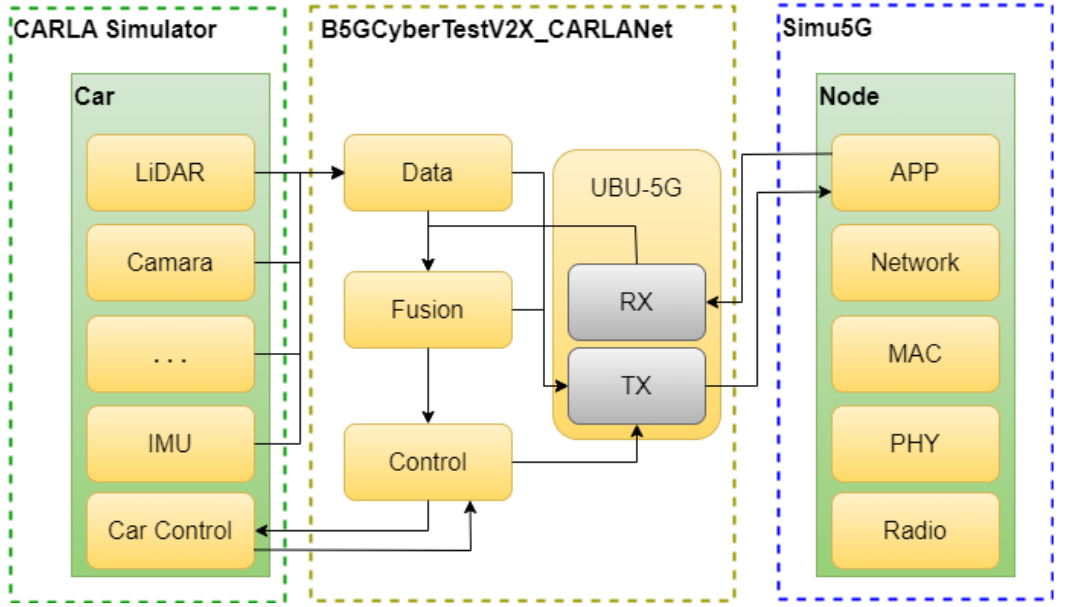
\includegraphics[width=0.85\textwidth]{parts/figuras/B5GCyberTestV2X_CARLANet.png}
    \caption{Block diagram depicting the B5GCyberTestV2X\_CARLANet architecture for integration between CARLA and Simu5G simulators. The diagram illustrates the data flow from vehicle sensors (LiDAR, Camera, IMU) through the central integration module to the Simu5G network simulation. Key components include the Data submodule for sensor acquisition, Fusion for data integration, Control for vehicle actuation, and the UBU-5G module containing RX/TX components that facilitate bidirectional communication with the Simu5G network stack.}
    \label{fig:B5GCyberTestV2X}
\end{figure*}

The communication between CARLA and B5GCyberTestV2X\_CARLANet continues to utilize TCP with Protocol Buffers (protobuf) for efficient data serialization, operating across ports 2000, 2001, and 2002. For the connection between B5GCyberTestV2X\_CARLANet and Simu5G, we continue to use the ZeroMQ service with the ZMTP protocol, working on top of the Carlanet project.

Our simulation workflow begins with the B5GCyberTestV2X\_CARLANet module initializing both simulators using configurations present in a single configuration file. During operation, an iterative cycle processes sensor data collection from CARLA vehicles, transmission of this data through the simulated 5G network, reception by other vehicles, fusion with local sensor data, and control actions based on the combined information. 

For the cooperative perception tests, Figure \ref{fig:B5GCyberTestV2X-use-case} depicts a use case that was implemented involving two autonomous vehicles communicating via V2V connections. In this scenario, Car 1 collects sensor data and transmits it to Car 2 through the simulated 5G network. Car 2 then fuses this data with its own sensor readings and executes control algorithms based on this combined information. 

\begin{figure*} [!ht]
    \centering
    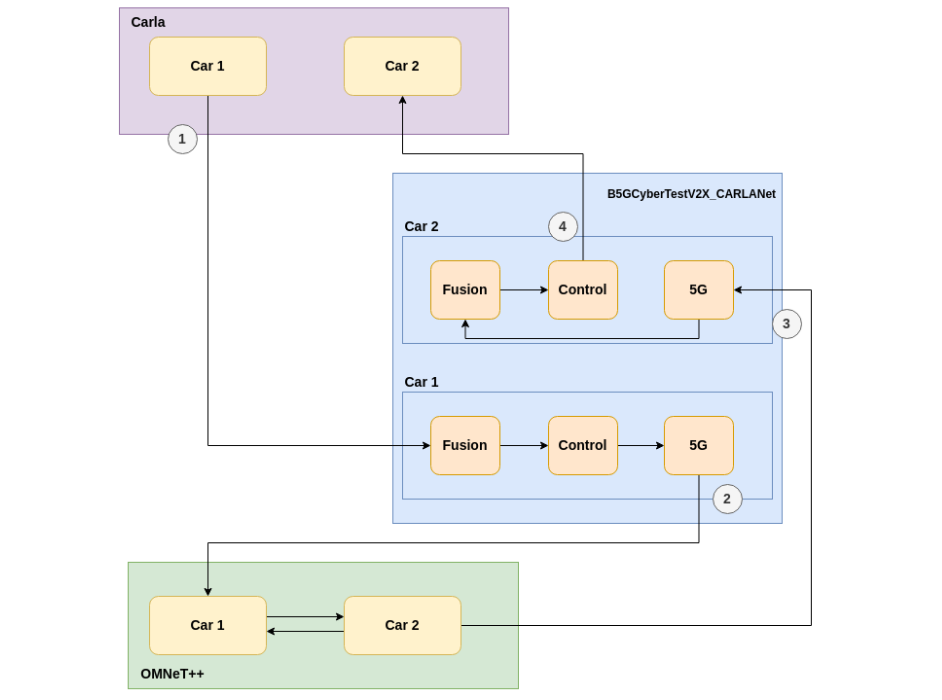
\includegraphics[width=0.95\textwidth]{parts/figuras/B5GCyberTestV2X_use_case.png}
    \caption{Block diagram of a shared perception use case in the B5GCyberTestV2X framework. 1. Car 1 in CARLA sends sensor data to the B5GCyberTestV2X\_CARLANet module; 2. data is transmitted to the OMNeT++ environment for network simulation; 3. Car 2 receives the processed data through its 5G module; 4. fusion and control components process the combined information to execute appropriate actions in the CARLA simulator.}
    \label{fig:B5GCyberTestV2X-use-case}
\end{figure*}

For monitoring and logging, each component of the system features its own implementation managed by the experiment code. Additionally, we used CARLA's Recorder feature to document events during simulation, allowing for detailed post-analysis and reproducibility of results. 

This integration framework represented a significant advancement in simulation for autonomous vehicle research in the cybersecurity domain. By combining traffic simulation with realistic 5G network modeling, the framework enables the testing of cooperative perception systems under various security scenarios.

\section{A Simulation Dataset for Vehicular Cybersecurity experiments}

Building on top of the developed data sharing framework, a series of standalone experiments were conducted to research vehicular cybersecurity, specifically focusing on Vehicle-to-Everything (V2X) communication security and spoofing attack detection.

This research addressed critical vulnerabilities in V2X systems where malicious actors can inject false information, disrupting traffic flow and compromising autonomous vehicle safety. The study combined hardware-level signal analysis (Direction of Arrival) with AI vision detection methods (YOLO V8) to develop a new method for detecting spoofing attacks and identifying the physical location of malicious senders.

\begin{figure*} [!ht]
    \centering
    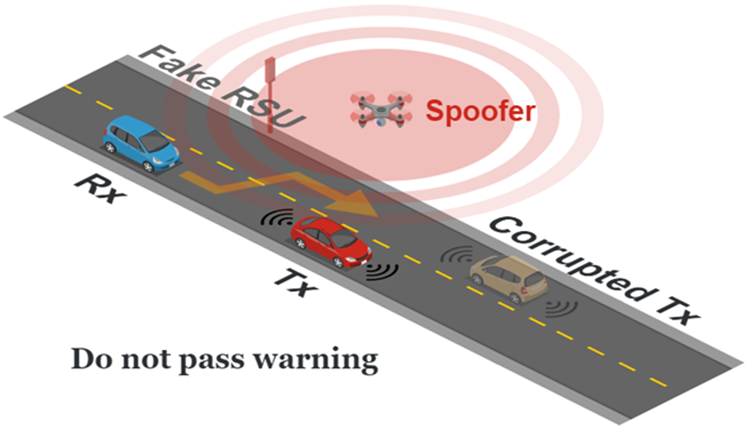
\includegraphics[width=0.5\textwidth]{parts/figuras/DoNotPassWarning.png}
    \caption{Do Not Pass Warning illustration depicting a drone-based attack where a malicious actor deploys a counterfeit roadside unit (RSU) to inject corrupted data into the vehicle network. The compromised signals disrupt V2X communications between the transmitting and receiving vehicles, creating unsafe conditions during passing maneuvers.}
    \label{fig:do-not-pass-warning}
\end{figure*}

Three autonomous driving scenarios were simulated using the CARLA simulator to generate the datasets. The first scenario, depicted in Figure \ref{fig:do-not-pass-warning}, "Do Not Pass Warning", represents a common highway situation where vehicles need to make overtaking decisions. This scenario involves communication between vehicles to ensure safe passing maneuvers, particularly critical when one vehicle needs to determine if there is sufficient time and space to overtake another vehicle safely.

The second scenario, "Vulnerable Road User Alerts at Blind Intersections", is illustrated in figure \ref{fig:vulnerable-road-user} addresses the challenge of detecting and responding to pedestrians at intersections with limited visibility. This scenario is particularly relevant it is a common occurrence in urban environments where buildings or other obstacles can obstruct a vehicle's direct line of sight.

\begin{figure*} [!ht]
    \centering
    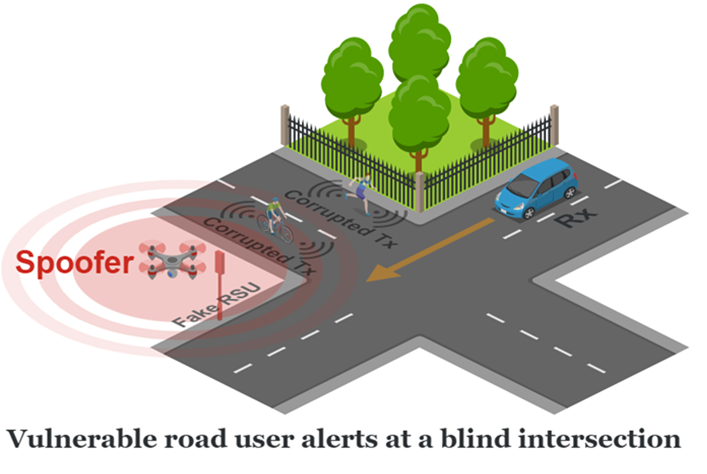
\includegraphics[width=0.5\textwidth]{parts/figuras/VulnerableRoadUserAlerts.png}
    \caption{Vulnerable Road User Alert system being compromised at a blind intersection. A drone-based attack using fake infrastructure signals disrupts critical safety communications between vehicles and pedestrians, creating heightened risk at an already visibility-limited crossing.}
    \label{fig:vulnerable-road-user}
\end{figure*}

The third scenario is called "Left Turn Assist" (available in figure \ref{fig:left-turn-assist}) focuses on the complex decision-making process required when vehicles execute left turns at intersections, requiring coordination and communication between multiple vehicles to prevent collisions.

\begin{figure*} [!ht]
    \centering
    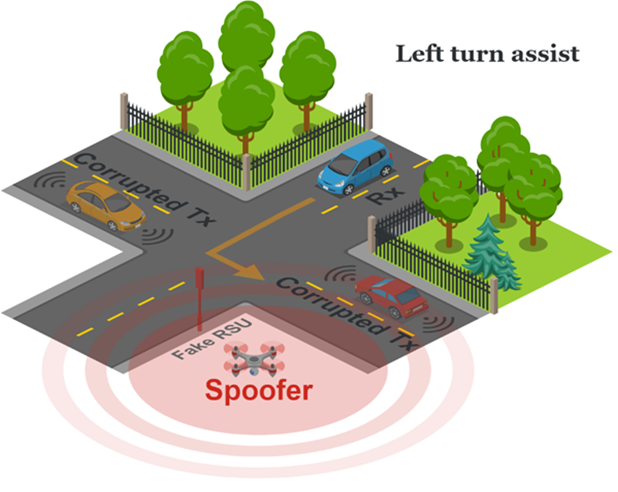
\includegraphics[width=0.5\textwidth]{parts/figuras/LeftTurnAssist.png}
    \caption{Left Turn Assist system compromised by a drone attack that uses counterfeit infrastructure signals to interfere with vehicle communications at the intersection. The spoofed data affects vehicles' ability to safely coordinate left turns, creating potential collision risks.}
    \label{fig:left-turn-assist}
\end{figure*}

For each of these scenarios, we collected two distinct subsets of data. The first subset captured normal operation data, where V2X communications functioned as intended, resulting in safe navigation and accident prevention. The second subset contained attack scenario data, where communications were compromised through spoofing attacks, leading to potential or actual accidents.

The dataset includes temporal sets of: vehicle position coordinates in three dimensions, vehicle orientation including pitch, yaw, and roll measurements, vehicle velocity vectors, camera captures from vehicle-mounted sensors, pedestrian position data where applicable, drone position and orientation data, and timestamp information for synchronization purposes.

In the Do Not Pass Warning scenario, data was collected from three vehicles and one drone. The normal operation subset demonstrated successful overtaking maneuvers where vehicles maintained safe distances based on accurate position and velocity information. The attack scenario subset revealed how spoofed location data led to unsafe passing decisions, resulting in collisions.

Figure \ref{fig:vulnerable-road-user-attack} shows the Vulnerable Road User scenario. In this scenario, we gathered data from two vehicles, one pedestrian, and one drone (the cyclist was considered a vehicle to the simulation). Normal operation data showed the system successfully detecting and responding to pedestrians at blind intersections. The attack scenario data documented instances where compromised sensor information resulted in vehicles failing to detect or appropriately respond to pedestrian presence.

\begin{figure*} [!ht]
    \centering
    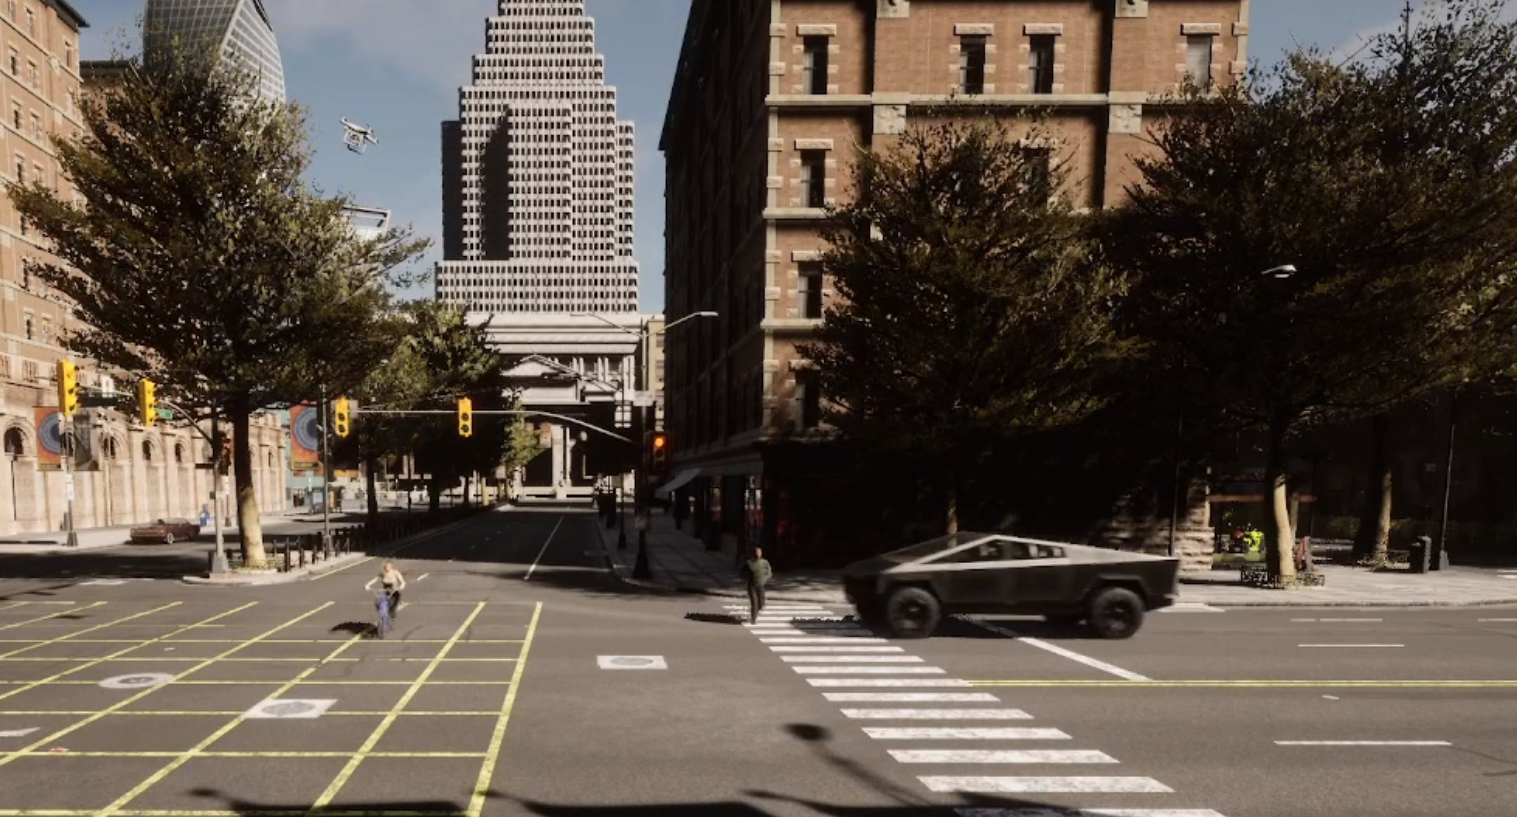
\includegraphics[width=0.8\textwidth]{parts/figuras/vulnerable-road-user.png}
    \caption{Simulation scenario of Vulnerable Road user use case, the vehicle can be seen about to collide with the pedestrian. The Spoofer drone can be seen in the sky, at the upper left corner of the image.}
    \label{fig:vulnerable-road-user-attack}
\end{figure*}

For the Left Turn Assist scenario, three vehicles and one drone were monitored. The normal operation subset captured successful left turn maneuvers enabled by proper V2V communication. The attack scenario subset illustrated how manipulated position and velocity data could lead to incorrect turn timing decisions and potential accidents. An example of attack situation can be seen in figure \ref{fig:left-turn-assist-attack}.

\begin{figure*} [!ht]
    \centering
    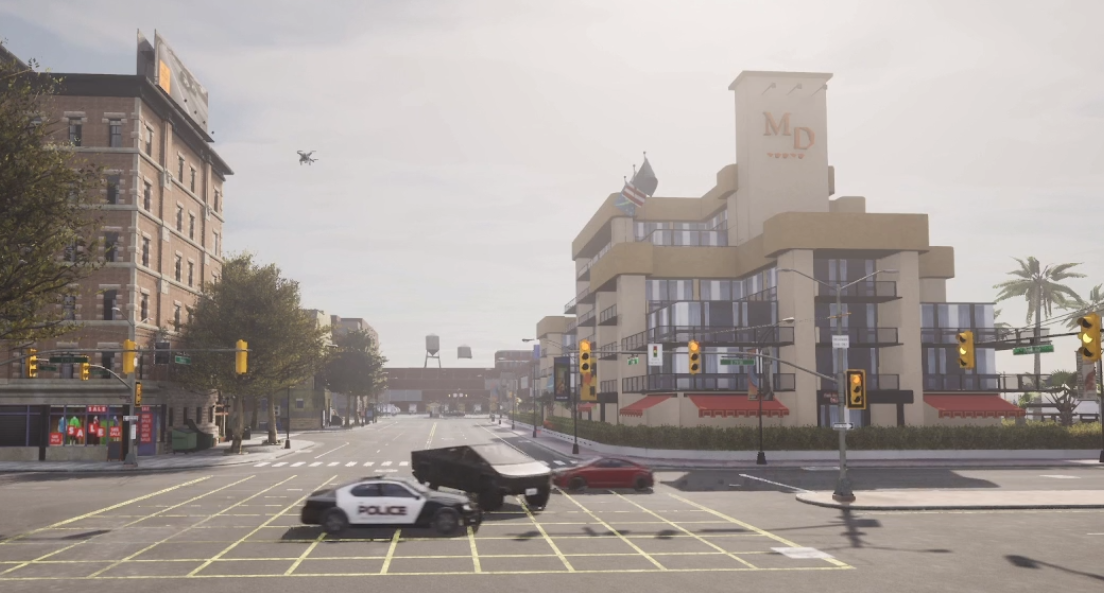
\includegraphics[width=0.8\textwidth]{parts/figuras/left-turn-assist-attack.png}
    \caption{A picture illustrating an attack in the Left Turn Assist scenario. The Tesla Cybertruck does a improperly timed left turn and ends up colliding with a police vehicle. The spoofer drone can be seen in the sky, close to the intersection.}
    \label{fig:left-turn-assist-attack}
\end{figure*}

The spatial and temporal data collected enabled accurate identification of malicious transmitters' physical locations through Direction of Arrival (DoA) estimation techniques. Furthermore, having both normal operations and attack scenarios helped training and validating our AI-based framework for attacker classification and countermeasure selection.

\section{Generating data for vision model finetuning}

To enable robust drone detection capabilities for identifying potential attackers, a specialized dataset was created for fine-tuning the YOLOv8 object detection model. The complete dataset comprises 4,824 annotated images focused on drone detection across various environments and conditions. This dataset was divided into a training set containing 3,877 images (80\% of the total) and a validation set of 947 images (20\% of the total).

A significant portion of the dataset was generated using the CARLA simulation environment. The data collection process involved placing stationary drones at strategic locations across different CARLA maps. Due to limitations in the simulation software's drone physics capabilities at the time of data collection, the drones remained in fixed positions throughout the collection process. Given the technical constraints of implementing new vehicle models in CARLA, a single drone model was utilized, the model and its dimensions inside the simulation are available in Figure \ref{fig:drone-dimensions}, though its appearance was varied through random color alterations to introduce visual diversity.

\begin{figure*} [!ht]
    \centering
    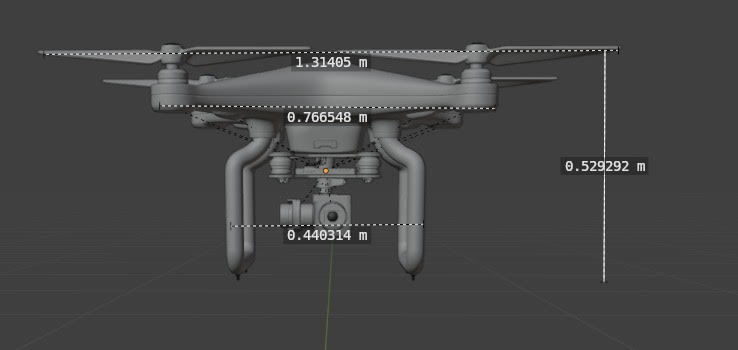
\includegraphics[width=0.8\textwidth]{parts/figuras/drone-dimensions.jpg}
    \caption{A picture of the drone model inserted in the simulation}
    \label{fig:drone-dimensions}
\end{figure*}

The image collection process in the simulation environment was conducted through automated vehicle routes with mounted cameras. These vehicles would navigate through the city environments, capturing images at approximately 0.3-second intervals. Each collection session lasted several minutes, during which simulation parameters were periodically randomized to create diverse scenarios. These parameters included weather conditions and time of day, ensuring the dataset captured a wide range of lighting conditions and atmospheric effects. One example can be seen in Figure \ref{fig:drone-simulation-capture}.

\begin{figure*} [!ht]
    \centering
    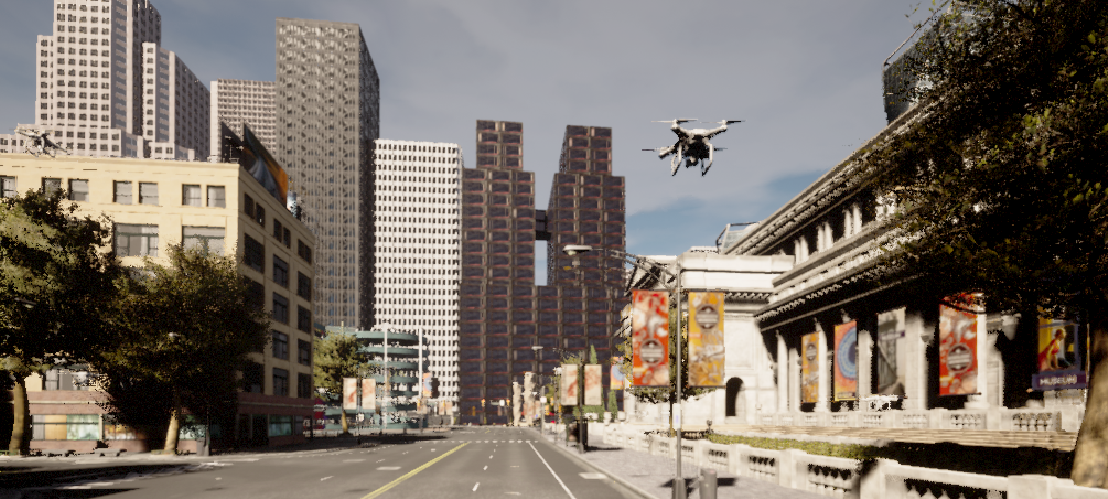
\includegraphics[width=0.8\textwidth]{parts/figuras/drone-simulation-capture.png}
    \caption{One of the raw images generated by the simulation for further annotation. A drone can be seen on the right with the sky as the background, while a second drone is a little harder to see is at the far left, with some buildings in the background.}
    \label{fig:drone-simulation-capture}
\end{figure*}

To supplement the simulated data and enhance the model's generalization capabilities, synthesized images showing drones in various lighting conditions and backgrounds were also incorporated in the dataset, as well as augmented versions of base images.

The annotation process required careful attention to detail and consistency. Each image received manual bounding box annotations indicating drone locations within the frame. A single-class labeling approach was maintained, focusing solely on drone detection, as this aligned with the specific need to identify potential attack sources. Annotation standards remained consistent across the entire dataset to ensure data quality.

The YOLOv8 model was trained with specific parameters optimized for this use case. The input format followed the NCHW standard (Batch, Channels, Height, Width) with image dimensions of 3×640×640 pixels. A batch size of 32 was used with the Adam optimizer and Cosine Annealing for learning rate scheduling. The initial learning rate was set to 0.005, gradually decreasing to 1.0e-05 throughout the training process. The model trained for 200 epochs to ensure proper convergence.

The performance metrics from the training process demonstrated strong detection capabilities. The model achieved a Mean Average Precision (mAP50) of approximately 0.9, indicating excellent accuracy in drone detection at the standard 50\% Intersection over Union (IoU) threshold. The more stringent mAP50-95 metric reached approximately 0.6, showing robust performance across varying IoU thresholds. Both precision and recall metrics stabilized near 0.9, indicating balanced performance in terms of false positives and false negatives.

The fine-tuned model became an important component of the larger spoofer detection framework. The high-accuracy drone detection capabilities were essential for identifying potential attack sources in V2X environments, complementing the signal processing approaches with visual confirmation of threat vectors. The model's reliable performance across various conditions enhanced the framework's overall ability to detect and respond to spoofing attacks in most real-world scenarios (at low lighting the results were not as good).

\section{Future Works: Security Challenges and Opportunities in V2X Cooperative Perception}

While significant progress has been made in establishing the B5GCyberTestV2X framework, training detection models, and simulating attack scenarios, several promising research directions remain unexplored. Building on our current foundation, several advanced research areas can be considered.

In the area of attack detection and mitigation, more sophisticated anomaly detection algorithms could be developed to identify vehicles purposely sharing incorrect location and speed data. This might include implementing real-time trust scoring mechanisms for data sources based on consistency and behavioral patterns. Additionally, adaptive countermeasures could be designed to automatically respond to different types of V2X attacks beyond the drone-based spoofing scenarios already simulated.

For resilient cooperative perception, future work could investigate predictive algorithms that maintain accurate environmental awareness during communication disruptions or jamming attacks. A critical challenge to address would be developing conflict resolution strategies when vehicle sensors and cooperative perception data provide contradictory information, such as when an object is placed in front of a vehicle in map data but not detected by onboard sensors.

Simulation capabilities could be further expanded to better model real-world scenarios. Additional network simulation tools might be integrated to model more complex attack vectors. The implementation of moving drone models with realistic physics would enhance the fidelity of aerial attack simulations. Furthermore, scenarios could be developed for testing system resilience against coordinated multi-vector attacks involving multiple malicious actors, providing insights into system vulnerabilities.

Looking to real-world applications, hardware-in-the-loop testing using the simulation framework connected to actual vehicle systems could be designed. Methodologies for transferring security insights from simulation to real-world V2X systems would be essential for practical implementation.

By exploring these research directions, the security and reliability of cooperative perception systems in autonomous driving could be further improved, making them more resilient against sophisticated cyber attacks and ensuring their robust operation in diverse real-world scenarios.
% ---

% ---
% Capítulo de conclusões
% ---
% ----------------------------------------------------------
\chapter{Results and Discussion}
% ----------------------------------------------------------

On the data collection part of this research, we evaluate the impact of a data aquisition model on AVs regarding local processing, storage and RAM usage (these parameters can also be used to estimate energy consumption). The experiment used the CARLA simulator in a client-server architecture and applied real-time data collection directly from the simulation server, as well as using application performance management tools.

Resulting data show that an extra data collection module at the vehicles offer a negligible 1.1\% increase in total memory usage  with direct sensor collection and a 2.6\% increase with application performance management (APM) data collection on the reference hardware.

The traffic monitoring experiment was designed to test the research question about the feasibility of traffic monitoring by the reuse of AV data for real-time traffic monitoring. Three "monitor vehicles" were placed in the simulation to collect GNSS and speedometer data. Two traffic conditions were simulated: light and heavy traffic. We show that it is feasible but we don't discuss network, identification and security concerns, important parameters in this topic, as that is reserved for future experiments.

The results obtained in the simulation by the proof-of-concept indicate that the proposed architecture could be applied in real world AVs; this form of data reuse can significantly improve ITS performance in its biggest challenges with minimal impact on current technology stack. Moreover, the reported experience with proof-of-concept allowed the identification of other promising research directions.

Our data transmission simulation expanded these concepts by integrating the CARLA simulator with communication network modeling through the B5GCyberTestV2X framework. This integration enabled realistic 5G network simulations for V2X communications, revealing that the bit rate required for basic cooperative perception (approximately 61.68 KB/s per vehicle) consumes only 0.049\% of a 5G antenna's capacity. This finding suggests that a single antenna could theoretically handle data from over 2000 vehicles simultaneously, confirming the technical feasibility of large-scale V2X implementations.

The development of the cooperative perception simulation framework for V2X security experiments represents a significant advancement in our research. By enabling vehicles to share sensor data through simulated 5G connections, we created a environment for testing cooperative perception under various security scenarios. The framework's modular architecture with separate components for data collection, fusion, and vehicle control facilitated detailed analysis of how vehicles can effectively share and utilize perception data.

Our cyber security experiments demonstrated the vulnerability of V2X systems to spoofing attacks. Through three detailed attack scenarios (Do Not Pass Warning, Vulnerable Road User Alerts, and Left Turn Assist), we simulated how malicious actors could compromise vehicle safety by injecting false information. The dataset created from these simulations provides valuable ground truth for developing and validating security countermeasures.

The vision model fine-tuning component of our research addressed the critical need for robust drone detection as part of a broader attack mitigation strategy. By creating a specialized dataset of 4,824 annotated images and finetuning a YOLOv8 model, we achieved high detection accuracy (mAP50 of approximately 0.9), demonstrating that visual confirmation can complement signal-based approaches in identifying potential threats.

Right now the amount of sensor data that would be transmitted, reflecting what we measured in usage of storage, is considerable. To tackle this problem, one of the possible research directions is the local pre-processing of the data in the vehicles prior to transmission and analyzing the impacts in relation to computing, like explored in \cite{THANDAVARAYAN2023103655}. Another involves proposing to improve the reliability of B5G in the presence of intermittent connectivity that can degrade data accuracy.

The B5GCyberTestV2X framework provides a starting platform for future research in V2X security, enabling more sophisticated simulations and the development of advanced defensive strategies. Through continued refinement of these tools and methodologies, the security and reliability of cooperative perception systems in autonomous driving could be significantly enhanced, making them more resilient against sophisticated cyber attacks and ensuring their robust operation in diverse real-world scenarios.

% The experiments conducted provide a foundation for understanding and furthering the capabilities of ITS technologies through AV data collection and traffic monitoring systems. The results encourage continued progression in cooperative perception and fusion technologies to address existing limitations within these systems. Further research may lead to the discovery of new avenues for smarter, more efficient transportation solutions.
% ---

% ------------------------------------------------------------------------
% ELEMENTOS PÓS-TEXTUAIS
% ------------------------------------------------------------------------
\postextual
% ------------------------------------------------------------------------

% ---
% Referências bibliográficas
% ---

\defbibheading{bibliography}[\bibname]{\chapter*{#1}}
\cleardoublepage
\phantomsection
\tocprintchapternonum
\addcontentsline{toc}{chapter}{\texorpdfstring{\MakeTextUppercase{\bibname}}{\bibname}}
\printbibliography
\markboth{}{}
% ---

%\defbibheading{bibliography}[\refname]{\section*{#1}\sectionmark{\refname}}

% ---
% Apêndices
% ---

\begin{apendicesenv}

% % Imprime uma página indicando o início dos apêndices
\partapendices

\IfStrEq*{\languagename}{english}{
% % ---
% % Resumo estendido. ara trabalhos escritos em inglês, é obrigatório conter um apêndice com resumo estendido em língua portuguesa.
% % ---
% \begin{refsection}

\chapter{Resumo Estendido em Língua Portuguesa}\label{appendix:pt_estendido}
\setlength{\absparsep}{18pt} % ajusta o espaçamento dos parágrafos do resumo
{\normalsize\noindent{\textbf{Título}: Título do trabalho em língua portuguesa}\\}
{\normalsize{\textbf{Autor:} Nome Completo do Autor}\\}
{\normalsize{\textbf{Orientador:} Nome Completo do Orientador}\\}
%{\setfonttimes\normalsize{\textbf{Coorientador:} Nome Completo do Coorientador}\\}
{\normalsize{\textbf{Programa de Pós-Graduação em Sistemas Mecatrônicos}}\\}
{\normalsize{\textbf{Brasília, 14 de setembro de 2022}}\\\\}
{\normalsize\noindent{\textbf{Palavras-chave:} Palavra chave 1. Palavra chave 2. Palavra chave 3. Palavra chave 4.}}

\vspace{-5mm}

\vspace{14pt}

\section*{Introdução}
Para dissertações ou teses em inglês, é necessário que o resumo em português seja no formato estendido. Trata-se de um formato com divisão própria de seções, como aqui exemplificado. A primeira seção deve ser denominada \emph{Introdução}.

O resumo estendido deve contar com uma lista própria de referências, citadas ao longo do resumo, como neste exemplo \cite{talbot2012}. Procure selecionar as referências mais importantes da sua lista principal. Pode usar a mesma 'chave' ou nome da referencia bibliografica usada no corpo do documento \cite{ibge1993}. É possível colocar as referências do resumo estendido em um arquivo bib diferente, mas não é necessário (no presente exemplo, as referências estão todas num só arquivo bib).

\section*{Materiais e Métodos}
O resumo estendido deve ter entre 4 e 6 páginas, pode incluir figuras e tabelas próprias, como no exemplo da Figura~\ref{fig:appendix_grafico}, mas lembre-se de usar "[]" após o "caption" e antes do "{}" para evitar que esta figura vá para a lista de figuras.

\begin{figure}[htb]
	\begin{center}
	    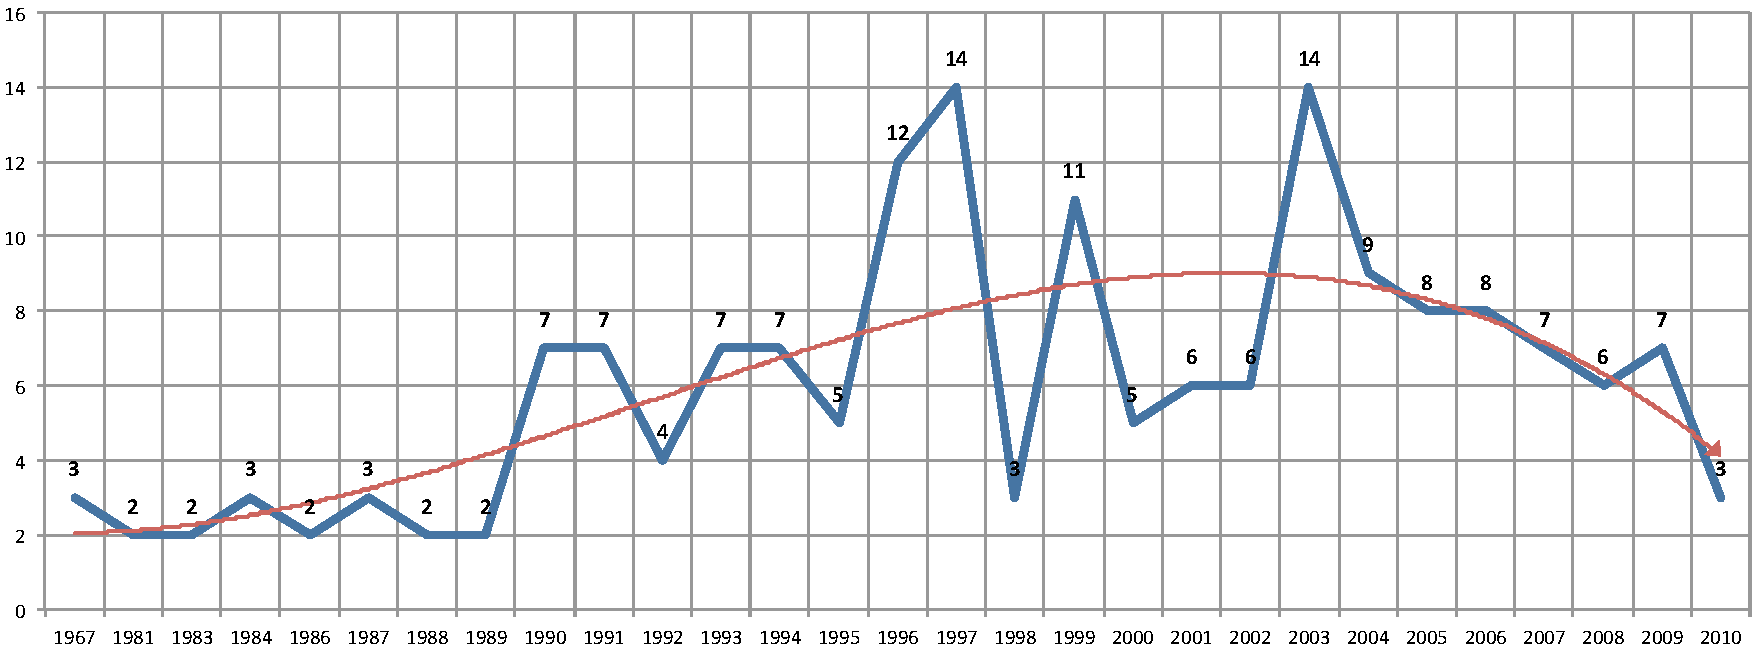
\includegraphics[scale=0.5]{img-grafico.pdf}
	\end{center}
	\caption[]{Este grafico novamente.}
    \label{fig:appendix_grafico}
	\legend{Fonte: \textcite[24]{araujo2012}}
\end{figure}

\section*{Resultados e Discussões}
Escreva aqui os resultados mais importantes. 

Os resultados da simulação numérica mostraram que ...

\section*{Conclusão}
A última seção deve ser denominada \emph{Conclusão}. 

Escreva aqui as conclusões.

% ---
% Referências bibliográficas do resumo estendido
% ---

{\let\clearpage\relax
\defbibheading{bibresumoestendido}[\bibname]{\section*{#1}}
\cleardoublepage
\phantomsection
\tocprintchapternonum
\addcontentsline{}{section}{\texorpdfstring{\MakeTextUppercase{\bibname}}{\bibname}}
\printbibliography[heading=bibresumoestendido, title={Referências}]
\markboth{}{}
}

\end{refsection}

 
% % ---
}



% ----------------------------------------------------------
\chapter{Research Source Code}
% ----------------------------------------------------------

All the source code for the present research was developed with the intent of reuse to enable easier code setups and scaffolding for quickly iterable research scenarios. As an example, sensors abstractions were created where a single function call would add different sensor sets at any vehicle or pedestrians at the simulation scenarios. Another example is the network simulations, where it is now possible to add a sensor to a vehicle, already knowing that data on that sensor will be transmitted, with a small number of configuration parameters.

The source code for the different research experiments is available in several github repositories (\url{https://github.com/av-data-research-group/carla-data-collection} for the first experiments, \url{https://github.com/carlanet/carlanetpp} for the network simulation framework and \url{https://github.com/aassilva/CarlaNetpp} for the network and attack experiments) and can be divided as following: 1. Code for data collection without network simulation; 2. Data collection with network simulation; 3. B5GCyberTestV2X code with interfaces for implementing vehicle control and data sharing funcionalities; 4. Spoofing attack scenarios experiment code; 5. Drone scenario generation.

Below we transcribe some files in an attempt to share the most meaningful part of the source code. The first file is a simple demonstration of the data collection process with the CARLA simulator.

\begin{lstlisting}[language=Python, caption={Basic starting code for a simple data collection example, using a single vehicle mounted with 2 cameras and a lidar sensor},label={code:starting}]

import carla
import random
import time


### Client

client = carla.Client('localhost', 2000)

client.set_timeout(10.0)
world = client.get_world()

# world.__dir__()
for map_name in client.get_available_maps():
    print(map_name)
world.get_map().name

# Load map
world = client.load_world("Town10HD_Opt")

# Get blueprint library and filter only cars
vehicle_blueprints = world.get_blueprint_library().filter('*vehicle*')
for idx, blueprint in enumerate(vehicle_blueprints):
    print(idx, blueprint.id)
    if idx == 10:
        break

### Add vehicle to world

# Get maps spawn points
spawn_points = world.get_map().get_spawn_points()

# Tesla Cybertruck
vehicle = world.try_spawn_actor(list(vehicle_blueprints)[26], random.choice(spawn_points))
print(vehicle)

vehicle_transform = vehicle.get_transform()
vehicle_transform.location.z += 2.0
world.get_spectator().set_transform(vehicle_transform)

### Add sensors to car

# time in seconds to collect data
SENSOR_TICK = 3

def get_cam_blueprint(world):
    cam_bp = world.get_blueprint_library().find('sensor.camera.rgb')
    cam_bp.set_attribute("image_size_x",str(400))
    cam_bp.set_attribute("image_size_y",str(300))
    cam_bp.set_attribute("fov",str(100))
    cam_bp.set_attribute("sensor_tick",str(SENSOR_TICK))
    return cam_bp


def get_lidar_blueprint(world):
    lidar_bp = world.get_blueprint_library().find('sensor.lidar.ray_cast')
    lidar_bp.set_attribute('sensor_tick', str(SENSOR_TICK))
    lidar_bp.set_attribute('channels', '64')
    lidar_bp.set_attribute('points_per_second', '1120000')
    lidar_bp.set_attribute('upper_fov', '30')
    lidar_bp.set_attribute('range', '100')
    lidar_bp.set_attribute('rotation_frequency', '100')
    return lidar_bp

camera_1_init_trans = carla.Transform(carla.Location(z=2.3))
camera_2_init_trans = carla.Transform(carla.Location(z=2.3), carla.Rotation(yaw=180))
lidar_init_trans = carla.Transform(carla.Location(z=3.0))

# creates camera and attaches it to the vehicle
camera_1_bp = get_cam_blueprint(world)
camera_2_bp = get_cam_blueprint(world)
camera_1 = world.spawn_actor(camera_1_bp, camera_1_init_trans, attach_to=vehicle)
camera_2 = world.spawn_actor(camera_2_bp, camera_2_init_trans, attach_to=vehicle)
camera_1.listen(lambda image: image.save_to_disk(f"sensors/camera_1/...{image.frame}.png"))
camera_2.listen(lambda image: image.save_to_disk(f"sensors/camera_2/...{image.frame}.png"))

# creates lidar and attaches it to the vehicle
lidar_bp = get_lidar_blueprint(world)
lidar = world.spawn_actor(lidar_bp, lidar_init_trans, attach_to=vehicle)
lidar.listen(lambda data: data.save_to_disk(f'sensors/lidar/...{data.frame}.ply'))

# Adds vehicle to Traffic manager
vehicle.set_autopilot(True)

# Faz o spectator seguir o carro
spectator = world.get_spectator()
while True:
    transform = camera_1.get_transform()
    transform.location.z += 2.0
    spectator.set_transform(transform)
    time.sleep(0.004)

# Remove o carro da simulação
vehicle.destroy()
\end{lstlisting}

The experiment code establishes a connection to the CARLA server running locally, allowing control of to the simulation. After connecting, it loads the high-definition urban environment "Town10HD\_Opt" and spawns a Tesla Cybertruck at a randomly selected spawn point. The script then configures and attaches multiple sensors to the vehicle: two RGB cameras positioned to capture front and rear views, and a high definition LiDAR sensor mounted on the roof. Each sensor is calibrated with specific parameters - the cameras are set with a 100 degree field of view and resolution of 400x300 pixels, while the LiDAR is configured with 64 channels, capturing 1.12 million points per second with a range of 100 meters. Please note that CPU and memory usage do scale with image and LIDAR definition.

The script implements a data collection pipeline where sensor outputs are automatically saved to disk at regular 3-second intervals. Camera images are stored as PNG files, while Lidar point clouds are saved as PLY files, organizing them by sensor type and frame number. This approach allows the creation of datasets capturing the vehicle's perspective as it navigates through the environment. The vehicle's movement is controlled by CARLA's built-in Traffic Manager through the autopilot function, ensuring realistic traffic behavior while data is being collected.

A spectator camera is programmed to follow the vehicle throughout the simulation, to provide the research team with a third-person view of the data collection process.

The following code represents a piece of the network data transmission capabilites.

\begin{lstlisting}[language=Python, caption={Simple data collection example, now using network simulation capabilities.},label={code:network}]
import random
import carla
import datetime
from carla import libcarla, ActorBlueprint
import traceback

from pycarlanet import CarlanetActor
from pycarlanet import CarlanetManager
from pycarlanet import CarlanetEventListener, SimulatorStatus

import math
import os
import pandas as pd

AUTO_PILOT = True
NUM_VEHICLES = 0

class B5GCyberTestV2X(CarlanetEventListener):
    def __init__(self, host, port):
        self.host = host
        self.port = port
        self.carlanet_manager = CarlanetManager(5555, self, log_messages=True)

        self.client = self.sim_world = self.carla_map = None
        self.carlanet_actors = dict()
        self._car = None
        self.remote_agent = RemoteAgent()

    def start_simulation(self):
        self.carlanet_manager.start_simulation()

    def omnet_init_completed(self, run_id, carla_configuration, user_defined) -> (SimulatorStatus, World):
        random.seed(carla_configuration['seed'])

        print(f'OMNeT world is completed with the id {run_id}')
        world = user_defined['carla_world']  # Retrieve from user_defined

        client: libcarla.Client = carla.Client(self.host, self.port)
        client.set_timeout(15)
        sim_world = client.load_world("Town01")
        #sim_world = client.load_world("Town10HD_Opt")
        
        settings = sim_world.get_settings()
        
        settings.synchronous_mode = False
        settings.fixed_delta_seconds = None
        settings.no_rendering_mode = False
        settings.fixed_delta_seconds = carla_configuration['carla_timestep']

        #sim_world.set_weather(carla.WeatherParameters.ClearNight)

        sim_world.apply_settings(settings)
        sim_world.tick()
        
        traffic_manager = client.get_trafficmanager()
        traffic_manager.set_synchronous_mode(False)
        traffic_manager.set_random_device_seed(
            carla_configuration['seed']
        )
        sim_world.tick()

        client.reload_world(False)  # Reload map keeping the world settings

        sim_world.tick()
        self.client, self.sim_world = client, sim_world
        self.carla_map = self.sim_world.get_map()

        return SimulatorStatus.RUNNING, self.sim_world

    def actor_created(self, actor_id: str, actor_type: str, actor_config) -> CarlanetActor:
        if actor_type == 'car':  # and actor_id == 'car_1':
            blueprint: ActorBlueprint = random.choice(
                self.sim_world.get_blueprint_library().filter(
                    "vehicle.tesla.model3"
                ))

            spawn_points = self.sim_world.get_map().get_spawn_points()
            # Attach sensors
            spawn_point = random.choice(spawn_points)
            print(blueprint)
            response = self.client.apply_batch_sync(
                [carla.command.SpawnActor(blueprint, spawn_point)]
            )[0]
            carla_actor: carla.Vehicle = self.sim_world.get_actor(response.actor_id)

            carla_actor.set_simulate_physics(True)
            if AUTO_PILOT:
                carla_actor.set_autopilot(True)

            carlanet_actor = CarlanetActor(carla_actor, True)
            self.carlanet_actors[actor_id] = carlanet_actor
            self._car = carlanet_actor

            self.vehicle = carla_actor

            self.sim_world.tick()

            #camera_sensor = TeleCarlaCameraSensor(2.2)
            #camera_sensor.attach_to_actor(self.sim_world, carla_actor)
            self.actor_id = actor_id
            
            # send spectator to camera position
            spectator = self.sim_world.get_spectator()
            transform = self.vehicle.get_transform()
            spectator.set_transform(transform)

            if NUM_VEHICLES > 0:
                vehicle_blueprints = self.sim_world.get_blueprint_library().filter(
                    '*vehicle*'
                )
                for _ in range(NUM_VEHICLES):
                    npc_vehicle = self.sim_world.try_spawn_actor(
                        list(vehicle_blueprints)[38], random.choice(spawn_points)
                    )
                    if npc_vehicle is None:
                        print("vehicle is none")
                    else:
                        npc_vehicle.set_autopilot(True)

            return carlanet_actor
        else:
            raise RuntimeError(f'I don\'t know this type {actor_type}')


    def carla_init_completed(self):
        super().carla_init_completed()

    def before_world_tick(self, timestamp) -> None:
        super().before_world_tick(timestamp)

    def carla_simulation_step(self, timestamp) -> SimulatorStatus:
        self.sim_world.tick()
        # Do all the things, save actors data
        if timestamp > 100:  # ts_limit
            return SimulatorStatus.FINISHED_OK
        else:
            return SimulatorStatus.RUNNING

    # get light control enum from int value
    @staticmethod
    def _str_to_light_control_enum(light_value):
        if light_value == '0':
            return carla.VehicleLightState.NONE
        elif light_value == '1':
            return carla.VehicleLightState.Position
        elif light_value == '2':
            return carla.VehicleLightState.Brake
        else:
            return carla.VehicleLightState.All
        
    # get int value from light control enum
    @staticmethod
    def _light_control_enum_to_str(light_enum):
        if light_enum == carla.VehicleLightState.NONE:
            return '0'
        elif light_enum == carla.VehicleLightState.Position:
            return '1'
        elif light_enum == carla.VehicleLightState.Brake:
            return '2'
        else:
            return '3'
        
    

    
    def standard_message(self, timestamp, user_defined_message) -> (SimulatorStatus, dict):
        # Handle the action of the actors in the world (apply_commands, calc_instruction)
        # es: apply_commands with id command_12 to actor with id active_actor_14
        if user_defined_message['msg_type'] == 'LIGHT_COMMAND':
            
            #convert enum value to enum
            next_light_state = self._str_to_light_control_enum(
                user_defined_message['light_next_state']
            )
            self._car.set_light_state(next_light_state)

            msg_to_send = {'msg_type': 'LIGHT_UPDATE',
                           'light_curr_state': self._light_control_enum_to_str(
                               self._car.get_light_state())    
                            }
            
            print("LIGHT CURR STATE: ", self._car.get_light_state(), '\n\n')
            return SimulatorStatus.RUNNING, msg_to_send
        
        elif user_defined_message['msg_type'] == 'LIGHT_UPDATE':
            curr_light_state = self._str_to_light_control_enum(
                user_defined_message['light_curr_state']
            )
            next_light_state = self.remote_agent.calc_next_light_state(
                curr_light_state
            )
            print("LIGHT CURR STATE: ", curr_light_state, "LIGHT NEXT STATE: ", next_light_state, '\n')

            msg_to_send = {'msg_type': 'LIGHT_COMMAND',
                           'light_next_state': self._light_control_enum_to_str(
                                next_light_state
                            )
                           }
            
            # GET locations and speed and save it to csv
            print("#" * 50)
            print("getting sensor data from car")
            self.remote_agent.process_vehicle_data(self.vehicle, self.carlanet_actors)

            ### CONTROL STAGE
            if not AUTO_PILOT:
                pass

            # send spectator to camera position
            spectator = self.sim_world.get_spectator()
            transform = self.vehicle.get_transform()
            spectator.set_transform(transform)

            return SimulatorStatus.RUNNING, msg_to_send
        else:
            raise RuntimeError(f"I don\'t know this type {user_defined_message['msg_type']}")

    def simulation_finished(self, status_code: SimulatorStatus):
        super().simulation_finished(status_code)

    def simulation_error(self, exception):
        traceback.print_exc()
        super().simulation_error(exception)


class RemoteAgent:

    def __init__(self):
        self.light_state = carla.VehicleLightState.NONE

    def calc_next_light_state(self, light_state: carla.VehicleLightState):
        return carla.VehicleLightState.NONE
    
    def generate_carla_nodes_positions(self, carlanet_actors):
        nodes_positions = []
        for actor_id, actor in carlanet_actors.items():
            transform: carla.Transform = actor.get_transform()
            velocity: carla.Vector3D = actor.get_velocity()
            position = dict()
            position['actor_id'] = actor_id
            position['position'] = [transform.location.x, transform.location.y, transform.location.z]
            position['rotation'] = [transform.rotation.pitch, transform.rotation.yaw, transform.rotation.roll]
            position['velocity'] = [velocity.x, velocity.y, velocity.z]
            position['is_net_active'] = actor.alive
            nodes_positions.append(position)
        return nodes_positions

    def process_vehicle_data(self, vehicle, carlanet_actors):
        file_name = f"sensors_high_traffic/gnss/vehicle-id-{vehicle.id}.csv"

        if not os.path.exists(f"sensors_high_traffic/gnss/"):
            os.makedirs(f"sensors_high_traffic/gnss/")

        positions_obj = self.generate_carla_nodes_positions(carlanet_actors)[0]
        x_speed = positions_obj["velocity"][0]
        y_speed = positions_obj["velocity"][1]
        z_speed = positions_obj["velocity"][2]
        speed = math.sqrt(x_speed**2 + y_speed**2 + z_speed**2)
        current_time = datetime.datetime.now()

        save_obj = [{
            "id": vehicle.id,
            "timestamp": str(current_time),
            "lat": positions_obj["position"][0],
            "long": positions_obj["position"][1],
            "alt": positions_obj["position"][2],
            "speed": speed
        }]

        if os.path.exists(file_name):
            df = pd.read_csv(file_name)
        else:
            df = None

        df_new_data = pd.DataFrame.from_dict(save_obj)

        if df is None:
            df_new_data.to_csv(file_name, index=False)
        else:
            df = pd.concat([df, df_new_data])
            df.to_csv(file_name, index=False)


if __name__ == '__main__':
    my_world = B5GCyberTestV2X('localhost', 2000)
    my_world.start_simulation()
\end{lstlisting}

This code implements a more advanced CARLA simulation that integrates with OMNET++/SIMU5G for network simulation capabilities. The architecture creates a bridge between two simulators: CARLA handles the vehicle physics, sensors, and urban environment, while SIMU5G/OMNET++ simulates 5G network communication between vehicles and infrastructure. The integration is managed through a custom CarlanetManager class that keeps the two simulators synced.

The main controller class, B5GCyberTestV2X, implements the CarlanetEventListener interface to set up the simulation environment and handle event callbacks between CARLA and OMNET++. It connects to the CARLA server on localhost, initializes a CarlanetManager for communicating with OMNET++, and sets up synchronization between the simulators with configurable timesteps. Unlike the previous code that used Town10HD\_Opt, this implementation loads the simpler Town01 map and configures traffic manager and weather settings accordingly.

For vehicle management, the code creates a Tesla Model 3 (instead of the Cybertruck in the previous example), places it at a random spawn point, and optionally enables autopilot through the AUTO\_PILOT flag. It can also spawn additional NPC vehicles based on the NUM\_VEHICLES setting. The network-vehicle integration is handled through a messaging system that supports two main message types: LIGHT\_COMMAND for controlling vehicle lights based on network commands, and LIGHT\_UPDATE for reporting the current light state back to the network.

Data collection is managed by the RemoteAgent class, which gathers vehicle telemetry data including position, velocity, and rotation. This data is saved to CSV files in a structured directory format, with each vehicle's information stored in a separate file with timestamps. The simulation maintains synchronization by having each simulator wait for the other before advancing to the next time step.

The key differences from the basic code include network integration through OMNET++/SIMU5G, more structured data collection with CSV storage, an event-based architecture using listeners for inter-simulator communication, and a more sophisticated vehicle control mechanism that can receive commands over the network. This implementation represents system where vehicle behavior can be influenced by network communications.

The next piece of code represents one of the use cases with data collection, now with the network and communication already abstracted in utility objects:

\begin{lstlisting}[language=Python, caption={Example Use case where data is collected from 3 cars and a drone may be used to perform attacks to the communication channels},label={code:use-case}]
import carla
import time

BAD_SCENARIO = True

from utils import (
    attach_all_sensors
)

def set_spectator(vehicle):
    spectator = world.get_spectator()
    transform = vehicle.get_transform()
    transform.location.z += 2.0
    spectator.set_transform(transform)

# entity used to preserve sensors in scope
simulation_actors = {}

client = carla.Client('localhost', 2000)
client.set_timeout(10.0)

# world = client.get_world()
world = client.load_world("Town01")
world.set_weather(carla.WeatherParameters.CloudyNoon)

time.sleep(5)

# Get blueprint library and filter only cars
# vehicle_blueprints = world.get_blueprint_library().filter('*vehicle*')
cyber_blueprints = world.get_blueprint_library().filter('vehicle.tesla.cybertruck')
c3_blueprints = world.get_blueprint_library().filter('vehicle.citroen.c3')
model_3_blueprints = world.get_blueprint_library().filter('vehicle.tesla.model3')
#drone_blueprint = world.get_blueprint_library().filter('vehicle.micro.microlino')[0]
drone_blueprint = world.get_blueprint_library().filter('vehicle.drone.drone1')[0]

# Get maps spawn points
spawn_points = world.get_map().get_spawn_points()

camera_init_trans = carla.Transform(carla.Location(z=2.7,x=1.0))
back_camera_init_trans = carla.Transform(carla.Location(z=2.7), carla.Rotation(yaw=180))
lidar_init_trans = carla.Transform(carla.Location(z=3.0))

# wanted positions: 181, 183, 177, 219
# wanted positions other lane: 65, 163

blueprint_list = [
    list(cyber_blueprints)[0],
    list(c3_blueprints)[0],
    list(model_3_blueprints)[0],
]
selected_locations = [181, 177, 163]
hero_list = []
for idx, location in enumerate(selected_locations):
    hero_n = world.try_spawn_actor(blueprint_list[idx], spawn_points[location])
    simulation_actors[f"vehicle_{hero_n.id}"] = hero_n
    if BAD_SCENARIO and idx == 2:
        attach_all_sensors(world, hero_n, simulation_actors, drone_attack=True)
    else:
        attach_all_sensors(world, hero_n, simulation_actors)
    hero_list.append(hero_n)


# set_spectator(hero_list[0])
print("Simulation actors:", simulation_actors)

if BAD_SCENARIO:
    # Malicious Drone
    drone_location = carla.Location(x=392.791443, y=107.608482, z=14.855516)
    drone_rotation = carla.Rotation(pitch=-27.212101, yaw=-89.532944, roll=-0.025725)
    drone_spawn_point = carla.Transform(drone_location, drone_rotation)
    drone_1 = world.try_spawn_actor(drone_blueprint, drone_spawn_point)
    drone_1.set_simulate_physics(False)


tm = client.get_trafficmanager()
tm_port = tm.get_port()

for hero_n in hero_list:
    hero_n.set_autopilot(True, tm_port)

if BAD_SCENARIO:
    tm.distance_to_leading_vehicle(hero_list[0], 0)
    tm.vehicle_percentage_speed_difference(hero_list[0], -80)
    tm.vehicle_percentage_speed_difference(hero_list[1], -75)
    tm.vehicle_percentage_speed_difference(hero_list[2], -80)
    tm.collision_detection(hero_list[0], hero_list[2], False)
    tm.collision_detection(hero_list[0], hero_list[1], False)
    tm.collision_detection(hero_list[2], hero_list[0], False)

spectator = world.get_spectator()
# Camera take - drone view
# spec_location = carla.Location(x=389.039062, y=102.294785, z=19.252405)
# spec_rotation = carla.Rotation(pitch=-31.561518, yaw=73.702972, roll=-0.018310)
# spectator.set_transform(carla.Transform(spec_location, spec_rotation))

# Camera take - lateral view
spec_location = carla.Location(x=377.332733, y=125.954506, z=35.793575)
spec_rotation = carla.Rotation(pitch=-54.568348, yaw=-0.546539, roll=-0.018311)
spectator.set_transform(carla.Transform(spec_location, spec_rotation))

starting_time = time.time()
print("current time", starting_time)
triggered = False
while True:
    # transform = camera_1.get_transform()
    # # transform.location.z += 1.0
    # spectator.set_transform(transform)
    time.sleep(0.1)

    ## DATA COLLECTION HAPPENS AUTOMATICALLY DURING THIS LOOP

    # find out locations
    spectator = world.get_spectator()
    print(spectator.get_transform())
\end{lstlisting}

This code creates a more scenario-focused CARLA simulation designed to test specific traffic situations, particularly centered around a potential malicious attack scenario. The implementation begins by connecting to a local CARLA server and loading the "Town01" map with cloudy noon weather conditions, allowing time for the world to properly initialize.

Rather than using random vehicles, this scenario have specific vehicle models - a Tesla Cybertruck, Citroen C3, and Tesla Model 3. The vehicles are placed at predetermined spawn points for reproducibility reasons (positions 181, 177, and 163) to create a controlled traffic scenario. Each vehicle is added to a "simulation\_actors" dictionary to maintain references and has sensors attached through the abstracted "attach\_all\_sensors" function, with special configuration for the third vehicle when the BAD\_SCENARIO flag is enabled.

We then implement a potentially hazardous situation when BAD\_SCENARIO is set to true. In this case, a drone actor is positioned at specific coordinates above the road and configured not to simulate physics (remaining stationary). The traffic manager is then set up with aggressive parameters: following distance for the first vehicle is minimized, all vehicles are instructed to drive much faster than normal, and collision detection between specific vehicle pairs is deliberately disabled.

The simulation's viewpoint is precisely positioned using a spectator camera at coordinates that provide a lateral view of the upcoming scenario. If the BAD\_SCENARIO is set to true, the drone will change the data that reaches vehicle 2 (the one trying to do the outtake in the road), making the data arrive with a big delay. With no visibility, vehicle 2 tries to outtake vehicle 1 and ends up coliding with vehicle 3.



% % ----------------------------------------------------------
\chapter{Códigos de programação}\label{apd:cdg}
% ----------------------------------------------------------

\section{Projeto do Controlador com Realimentação de Estados}
\lstinputlisting[language=Matlab,caption=Código de Matlab]{parts/codigos/controle.m}

\section{Exemplo de teste em Malha Fechada com Rampa}
\lstinputlisting[language=Python,caption=Código de Python]{parts/codigos/controleSmithPredictor.py}

\section{Redução modal}
\lstinputlisting[language=Julia,caption=Código de Julia]{parts/codigos/ModalReduction.jl}

\end{apendicesenv}

% ---

% ---
% Anexos
% ---

% \begin{anexosenv}

% % Imprime uma página indicando o início dos anexos
% \partanexos

% % ----------------------------------------------------------
\chapter{Figuras de exemplo}
% ----------------------------------------------------------

% Fonte: https://tex.stackexchange.com/a/231741/91816 (Gonzalo Medina)

\noindent\includegraphics[width=3cm]{example-image-a}\qquad
\includegraphics[width=3cm]{example-image-golden}\qquad
\includegraphics[width=3cm]{example-grid-100x100pt}

\noindent\includegraphics[height=5cm]{example-image-b} 

\noindent\includegraphics[scale=0.5]{example-image-c} 

\noindent\includegraphics[width=3cm]{example-image} 

% % ----------------------------------------------------------
\chapter{Logo LaTeX}
% ----------------------------------------------------------

\vfill

\begin{center}
{\fontsize{50pt}{800pt}\selectfont \LaTeX}\
\end{center}

\vfill

\begin{center}
{\color{azulunb}\fontsize{50pt}{800pt}\selectfont \LaTeX}\
\end{center}

\vfill

\begin{center}
{\color{verdeunb}\fontsize{50pt}{800pt}\selectfont \LaTeX}\
\end{center}

\vfill

% \end{anexosenv}

\end{document}